% Created with jtex v.0.1.15
\documentclass{article}
\usepackage{arxiv}

\usepackage[utf8]{inputenc} % allow utf-8 input
\usepackage[T1]{fontenc}    % use 8-bit T1 fonts
\usepackage{hyperref}       % hyperlinks
\usepackage{url}            % simple URL typesetting
\usepackage{datetime}       % show dates in the title block
\usepackage{booktabs}       % professional-quality tables
\usepackage{amsfonts}       % blackboard math symbols
\usepackage{nicefrac}       % compact symbols for 1/2, etc.
\usepackage{microtype}      % microtypography
\usepackage{graphicx}
\usepackage{natbib}
\usepackage{doi}
\usepackage{xcolor}

%%%%%%%%%%%%%%%%%%%%%%%%%%%%%%%%%%%%%%%%%%%%%%%%%%
%%%%%%%%%%%%%%%%%%%%  imports  %%%%%%%%%%%%%%%%%%%
\usepackage{amsmath}
%%%%%%%%%%%%%%%%%  math commands  %%%%%%%%%%%%%%%%
\newcommand{\DiscFac}{\beta}
\newcommand{\utilFunc}{\mathrm{u}}
\newcommand{\VFunc}{\mathrm{V}}
\newcommand{\Leisure}{Z}
\newcommand{\tShk}{\xi}
\newcommand{\util}{u}
\newcommand{\tShkEmp}{\theta}
\newcommand{\BLev}{B}
\newcommand{\CLev}{C}
\newcommand{\Ex}{\mathbb{E}}
\newcommand{\CRRA}{\rho}
\newcommand{\labShare}{\nu}
\newcommand{\leiShare}{\zeta}
\newcommand{\h}{h}
\newcommand{\bRat}{b}
\newcommand{\leisure}{z}
\newcommand{\cRat}{c}
\newcommand{\PLev}{P}
\newcommand{\vFunc}{\mathrm{v}}
\newcommand{\Rfree}{\mathsf{R}}
\newcommand{\riskyshare}{\varsigma}
\newcommand{\PGro}{\Gamma}
\newcommand{\labor}{\ell}
\newcommand{\aRat}{a}
\newcommand{\mRat}{m}
\newcommand{\Rport}{\mathbb{R}}
\newcommand{\Risky}{\mathbf{R}}
\newcommand{\risky}{\mathbf{r}}
\newcommand{\vOpt}{\tilde{\mathfrak{v}}}
\newcommand{\vEnd}{\mathfrak{v}}
\newcommand{\vE}{{v}^{e}}
\newcommand{\vOptAlt}{\grave{\tilde{\mathfrak{v}}}}
\newcommand{\q}{\koppa}
\newcommand{\cEndFunc}{\mathfrak{c}}
\newcommand{\cE}{\cRat^{e}}
\newcommand{\xRat}{x}
\newcommand{\aMat}{[\mathrm{a}]}
\newcommand{\mEndFunc}{\mathfrak{m}}
\newcommand{\mE}{\mRat^{e}}
\newcommand{\mMat}{[\mathrm{m}]}
\newcommand{\tShkMat}{[\mathrm{\tShkEmp}]}
\newcommand{\zEndFunc}{\mathfrak{z}}
\newcommand{\lEndFunc}{\mathfrak{l}}
\newcommand{\bEndFunc}{\mathfrak{b}}
\newcommand{\bE}{\bRat^{e}}
\newcommand{\nRat}{n}
\newcommand{\dRat}{d}
\newcommand{\gFunc}{\mathrm{g}}
\newcommand{\xFer}{\chi}
\newcommand{\lRat}{l}
\newcommand{\wFunc}{\mathrm{w}}
\newcommand{\dEndFunc}{\mathfrak{d}}
\newcommand{\nEndFunc}{\mathfrak{n}}
\newcommand{\uFunc}{\mathrm{u}}
\newcommand{\TFunc}{\mathrm{T}}
\newcommand{\UFunc}{\mathrm{U}}
\newcommand{\WFunc}{\mathrm{W}}
\newcommand{\yRat}{y}
\newcommand{\Retire}{\mathbb{R}}
\newcommand{\Work}{\mathbb{W}}
\newcommand{\error}{\epsilon}
\newcommand{\err}{z}
\newcommand{\kapShare}{\alpha}
\newcommand{\kap}{k}
\newcommand{\cTarg}{\check{c}}
\newcommand{\Decision}{\mathbb{D}}
\newcommand{\Prob}{\mathbb{P}}
%%%%%%%%%%%%%%%%%%%%%%%%%%%%%%%%%%%%%%%%%%%%%%%%%%

\hypersetup{colorlinks = true,
    linkcolor = purple,
    urlcolor  = blue,
    citecolor = cyan,
    anchorcolor = black}

\title{EGMⁿ: The Sequential Endogenous Grid Method}

\newdate{articleDate}{27}{6}{2023}
\date{\displaydate{articleDate}}

\makeatletter
\let\@fnsymbol\@arabic
\makeatother

\author{    Alan Lujan    \footnotemark[1]\\
    Ohio State University\\Econ-ARK\\        }

% Uncomment to override  the `A preprint' in the header
\renewcommand{\headeright}{Economics}
\renewcommand{\undertitle}{}
\renewcommand{\shorttitle}{EGMⁿ}

%% Add PDF metadata to help others organize their library
%% Once the PDF is generated, you can check the metadata with
%% $ pdfinfo template.pdf
\hypersetup{
    pdftitle={\@title},
    pdfsubject={},
    pdfauthor={\@author},
    pdfkeywords={endogenous grid method,stochastic dynamic programming,machine learning,gaussian process regression},
    addtopdfcreator={Written in Curvenote}
}

\begin{document}
    \maketitle
            \footnotetext[1]{Correspondence to: alanlujan91@gmail.com}

        \begin{abstract}
    Heterogeneous agent models with multiple decisions are often solved using inefficient grid search methods that require many evaluations and are slow.
This paper provides a novel method for solving such models using an extension of the Endogenous Grid Method (EGM) that uses Gaussian Process Regression (GPR) to interpolate functions on unstructured grids.
First, I propose an intuitive and strategic procedure for decomposing a problem into subproblems which allows the use of efficient solution methods.
Second, using an exogenous grid of post-decision states and solving for an endogenous grid of pre-decision states that obey a first-order condition greatly speeds up the solution process.
Third, since the resulting endogenous grid can often be non-rectangular at best and unstructured at worst, GPR provides an efficient and accurate method for interpolating the value, marginal value, and decision functions.
Applied sequentially to each decision within the problem, the method is able to solve heterogeneous agent models with multiple decisions in a fraction of the time and with less computational resources than are required by standard methods currently used.
Software to reproduce these methods is available under the \href{https://econ-ark.org/}{\texttt{Econ-ARK/HARK}} project for the \texttt{python} programming language.
    \end{abstract}

        \keywords{endogenous grid method, stochastic dynamic programming, machine learning, gaussian process regression}

    I would like to thank Chris Carroll and Simon Scheidegger for their helpful comments and suggestions. The remaining errors are my own. All figures and other numerical results were produced using the \href{https://econ-ark.org/}{\texttt{Econ-ARK/HARK}} toolkit (\citet{Carroll2018}). Additional libraries used in the production of this paper include but are not limited to: \href{https://www.scipy.org/}{\texttt{scipy}} (\citet{Virtanen2020}), \href{https://www.numpy.org/}{\texttt{numpy}} (\citet{Harris2020}), \href{https://numba.pydata.org/}{\texttt{numba}} (\citet{Lam2015}), \href{https://cupy.dev/}{\texttt{cupy}} (\citet{Okuta2017}), \href{https://scikit-learn.org/}{\texttt{scikit-learn}} (\citet{Pedregosa2011}), \href{https://pytorch.org/}{\texttt{pytorch}} (\citet{Paszke2019}), and \href{https://gpytorch.ai/}{\texttt{gpytorch}} (\citet{Gardner2018})

\section{Introduction}\label{introduction}

% Introduce the topic by providing a brief overview of the issue and why it is important to study it.

% Identify the research question: Clearly state the research question or problem being addressed in the current study.
%  Provide context: Explain why the topic is important to study and what gap in the existing knowledge the current study aims to fill.
%  Summarize the existing literature: Briefly describe what is currently known about the topic, including any relevant studies or theories that have been previously published.
%  Highlight the limitations of previous research: Identify any limitations or gaps in the existing literature and explain how the current study will address these limitations.
%  Provide a rationale for the study: Explain why the current study is needed and why it is a significant contribution to the existing knowledge on the topic.

% Use only the first paragraph to state the question and describe its importance. Don't weave
%  around, be overly broad, or use prior literature to motivate it (the question is not important
%  because so many papers looked at this issue before!).

Macroeconomic modeling aims to describe a complex world of agents interacting with each other and making decisions in a dynamic setting. The models are often very complex, require strong underlying assumptions, and use a lot of computational power to solve. One of the most common methods to solve these complex problems is using a grid search method to solve the model. The Endogenous Grid Method (EGM) developed by \citet{Carroll2006} allows dynamic optimization problems to be solved in a more computationally efficient and faster manner than the previous method of convex optimization using grid search. Many problems that before took hours to compute became much easier to solve and allowed macroeconomists and computational economists to focus on estimation and simulation.
However, the Endogenous Grid Method is limited to a few specific classes of problems. Recently, the classes of problems to which EGM can be applied have been expanded\footnote{\citet{Barillas2007, Maliar2013, Fella2014, White2015, Iskhakov2017}, among others.}, but with every new method comes a new set of limitations.
This paper introduces a new approach to EGM in a multivariate setting. The method is called Sequential EGM (or EGM$^n$) and introduces a novel way of breaking down complex problems into a sequence of simpler, smaller, and more tractable problems, along with an exploration of new multidimensional interpolation methods that can be used to solve these problems.

\subsection{Literature Review}\label{Literature Review}

% Summarize the existing literature on the topic and highlight any gaps or limitations in the current research.

% Then use the second paragraph for a summary of the most relevant literature
%  (not a full Section!). Hint: use present tense, to be consistent. "Smith (1986) presents a similar model, ..."

\citet{Carroll2006} first introduced the Endogenous Grid Method as a way to speed up the solution of dynamic stochastic consumption-savings problems. The method consists of starting with an exogenous grid of post-decision states and using the inverse of the first-order condition to find the optimal consumption policy that rationalizes such post-decision states. Given the optimal policy and post-decision states, it is straightforward to calculate the initial pre-decision state that leads to the optimal policy. Although this method is certainly innovative, it only applied to a model with one control variable and one state variable. \citet{Barillas2007} further extend this method by including more than one control variable in the form of a labor-leisure choice, as well as a second state variable for stochastic persistence.

\citet{Hintermaier2010} introduce a model with collateral constraints and non-separable utility and solve using an EGM method that allows for occasionally binding constraints among endogenous variables. \citet{Jorgensen2013} evaluates the performance of the Endogenous Grid Method against other methods for solving dynamic stochastic optimization problems and finds it to be fast and efficient. \citet{Maliar2013} develop the Envelope Condition Method based on a similar idea as the Endogenous Grid Method, avoiding the need for costly numerical optimization and grid search. However, their model is limited to infinite horizon problems as it is a forward solution method.

Further development into a multivariate Endogenous Grid Method expanded the ability of researchers to solve models efficiently. \citet{White2015} formally characterized the conditions for the Endogenous Grid Method and developed an interpolation method for structured non-rectilinear, or curvilinear, grids. \citet{Iskhakov2015} additionally establishes conditions for solving multivariate models with EGM, requiring the invertibility of a triangular system of first-order conditions. \citet{Ludwig2018} also develops a novel interpolating method using Delaunay triangulation of the resulting unstructured endogenous grid. However, the authors show that the gains from avoiding the grid search method are often offset by the costly construction of the triangulation.

For the papers discussed above, continuity and smoothness of the value and first-order conditions are strict requirements. \citet{Fella2014} first introduced a method to solve non-convex problems using the Endogenous Grid Method. The idea is based on evaluating necessary but not sufficient candidates for the first-order condition in overlapping regions of the state space. \citet{Arellano2016} use the Envelope Condition Method to solve a sovereign default risk model with similar efficiency gains to EGM. \citet{Iskhakov2017} further advances the methodology by using extreme errors to solve discrete choice problems with Endogenous Grid Method. These methods however were only applied to a single control variable and a single state variable. \citet{Druedahl2017} introduces the $G2EGM$ to handle non-convex problems with more than 1 control variable and more than 1 state variable. This method is also capable of handling occasionally binding constraints which previous multivariate EGM methods were not.

\citet{Clausen2020} formalize the applicability of the Endogenous Grid Method and its extensions to discrete choice models and discuss the nesting of problems to efficiently find accurate solutions. \citet{Druedahl2021} similarly suggest the nesting of problems to efficiently use the Endogenous Grid Method within problems with multiple control variables. However, while these nested methods reduce the complexity of solving these models, they often still require grid search methods as is the case with \citet{Druedahl2021}.

% Finally, this paper contributes to the literature of solving dynamic optimization problems using machine learning tools. {cite:t}`Scheidegger2019` introduce the use of Gaussian Process Regression to compute global solutions for high-dimensional dynamic stochastic problems. {cite:t}`Maliar2021` use non-linear regression and neural networks to estimate systems of equations that characterize dynamic economic models.

\subsection{Research Question}\label{Research Question}

% Clearly state the research question or problem being addressed in the current study.

% Next, while still on page one, the third paragraph must begin: "The purpose of this paper is ...",
%  and summarize what you actually do. (Paragraphs 2 and 3 could be reversed.)

The purpose of this paper is to describe a new method for solving dynamic optimization problems efficiently and accurately while avoiding convex optimization and grid search methods with the use of the Endogenous Grid Method and first-order conditions. The method is called Sequential EGM (or EGM$^n$) and introduces a novel way of breaking down complex problems into a sequence of simpler, smaller, and more tractable problems, along with an exploration of new multidimensional interpolation methods that can be used to solve these problems. This paper also illustrates an example of how Sequential EGM can be used to solve a dynamic optimization problem in a multivariate setting.

\subsection{Methodology}\label{Methodology}

% Briefly describe the research methodology used in the study, including any data sources, econometric techniques, or other methods used.

The sequential Endogenous Grid Method consists of 3 major parts: First, the problem to be solved should be broken up into a sequence of smaller problems that themselves don't add any additional state variables or introduce asynchronous dynamics with respect to the uncertainty. If the problem is broken up in such a way that uncertainty can happen in more than one period, then the solution to this sequence of problems might be different from the aggregate problem due to giving the agent additional information about the future by realizing some uncertainty. Second, I evaluate each of the smaller problems to see if they can be solved using the Endogenous Grid Method. This evaluation is of greater scope than the traditional Endogenous Grid Method, as it allows for the resulting exogenous grid to be non-regular. If the subproblem can not be solved with EGM, then convex optimization is used. Third, if the exogenous grid generated by the EGM is non-regular, then I use a multidimensional interpolation method that takes advantage of machine learning tools to generate an interpolating function. Solving each subproblem in this way, the sequential Endogenous Grid Method is capable of solving complex problems that are not solvable with the traditional Endogenous Grid Method and are difficult and time-consuming to solve with convex optimization and grid search methods.

\subsection{Contributions}\label{Contributions}

% Discuss how the current study contributes to the existing literature and what new insights it provides.

% That sets you up for the fourth paragraph, which lists "The contributions of
%  this work" – relative to that prior literature. Clarify what you do that's different

The Sequential Endogenous Grid Method is capable of solving multivariate dynamic optimization problems in an efficient and fast manner by avoiding grid search. This should allow researchers and practitioners to solve more complex problems that were previously not easily accessible to them, but more accurately capture the dynamics of the macroeconomy. By using advancements in machine learning techniques such as Gaussian Process Regression, the Sequential Endogenous Grid Method is capable of solving problems that were not previously able to be solved using the traditional Endogenous Grid Method. In particular, the Sequential Endogenous Grid Method is different from NEGM in that it allows for using more than one Endogenous Grid Method step to solve a problem, avoiding costly grid search methods to the extent that the problem allows.

Additionally, the Sequential Endogenous Grid Method often sheds light on the problem by breaking it down into a sequence of simpler problems that were not previously apparent. This is because intermediary steps in the solution process generate value and marginal value functions of different pre- and post-decision states that can be used to understand the problem better.

% The fifth paragraph then summarizes your results. Tell the answer, so they know what to expect,
%  and how to think about each step along the way, what's driving your results.

\subsection{Outline}\label{Outline}

% Provide a brief overview of the results and conclusions that will be presented in the article.
%  In the sixth and final paragraph, as an aid to the reader, plot the course for the rest of the paper.
%  "The first Section below presents a theoretical model that can be used to generate specific
%  hypotheses. Then [Section %s](#method) presents the econometric model, ..."

Section~\ref{method} presents a basic model that illustrates the sequential Endogenous Grid Method in one dimension. Then Section~\ref{multdim} introduces a more complex method with two state variables to demonstrate the use of machine learning tools to generate an interpolating function. In Section~\ref{multinterp} I present the unstructured interpolation methods using machine learning in more detail. Section~\ref{conditions} discusses the theoretical requirements to use the Sequential Endogenous Grid Method. Finally, Section~\ref{conclusion} concludes with some limitations and future work.

\section{The Sequential Endogenous Grid Method}\label{method}

\subsection{A basic model}\label{A basic model}

The baseline problem which I will use to demonstrate the Sequential Endogenous Grid Method (EGM$^n$) is a discrete time version of \citet{Bodie1992} where a consumer has the ability to adjust their labor as well as their consumption in response to financial risk. The objective consists of maximizing the present discounted lifetime utility of consumption and leisure.

\begin{equation}
\VFunc_0(\BLev_0, \tShkEmp_0) = \max \Ex_{t} \left[ \sum_{n = 0}^{T-t} \DiscFac^{n} \utilFunc(\CLev_{t+n}, \Leisure_{t+n})  \right]
\end{equation}

In particular, this example makes use of a utility function that is based on Example 1 in the paper, which is that of additively separable utility of labor and leisure as

\begin{equation}
\utilFunc(\CLev, \Leisure) = \util(\CLev) + \h(\Leisure) = \frac{C^{1-\CRRA}}{1-\CRRA} + \labShare^{1-\CRRA} \frac{\Leisure^{1-\leiShare}}{1-\leiShare}
\end{equation}

where the term $\labShare^{1 -\CRRA}$ is introduced to allow for a balanced growth path as in \citet{Mertens2011}. The use of additively separable utility is ad-hoc, as it will allow for the use of multiple EGM steps in the solution process, as we'll see later.

This model represents a consumer who begins the period with a level of bank balances $\bRat_{t}$ and a given wage offer $\tShkEmp_{t}$. Simultaneously, they are able to choose consumption, labor intensity, and a risky portfolio share with the objective of maximizing their utility of consumption and leisure, as well as their future wealth.

The problem can be written in normalized recursive form\footnote{As in \citet{Carroll2009}, where the utility of normalized consumption and leisure is defined as

\begin{equation}
\utilFunc(\cRat_{t}, \leisure_{t}) = \PLev_{t}^{1-\CRRA} \frac{\cRat_{t}^{1-\CRRA}}{1-\CRRA} + (\labShare\PLev_{t})^{1-\CRRA} \frac{\leisure_{t}^{1-\leiShare}}{1-\leiShare}
\end{equation}} as

\begin{equation}
\begin{split}
    \vFunc_{t}(\bRat_{t}, \tShkEmp_{t}) & = \max_{\{\cRat_{t},
      \leisure_{t}, \riskyshare_{t}\}} \utilFunc(\cRat_{t}, \leisure_{t}) +
    \DiscFac \Ex_{t} \left[ \PGro_{t+1}^{1-\CRRA}
      \vFunc_{t+1} (\bRat_{t+1},
      \tShkEmp_{t+1}) \right] \\
    & \text{s.t.} \\
    \labor_{t} & = 1 - \leisure_{t} \\
    \mRat_{t} & = \bRat_{t} + \tShkEmp_{t}\labor_{t} \\
    \aRat_{t} & = \mRat_{t} - \cRat_{t} \\
    \Rport_{t+1} & = \Rfree + (\Risky_{t+1} - \Rfree)
    \riskyshare_{t} \\
    \bRat_{t+1} & = \aRat_{t} \Rport_{t+1} / \PGro_{t+1}
  \end{split}
\end{equation}

in which $\labor_{t}$ is the time supplied to labor net of leisure, $\mRat_{t}$ is the market resources totaling bank balances and labor income, $\aRat_{t}$ is the amount of saving assets held by the consumer, and $\riskyshare_{t}$ is the risky share of assets, which induce a $\Rport_{t+1}$ return on portfolio that results in next period's bank balances $\bRat_{t+1}$ normalized by next period's permanent income $\PGro_{t+1}$.

% \begin{equation}
%   \begin{split}
%    \vFunc_{t}(\bRat_{t}, \tShkEmp_{t}) & = \max_{\cRat_{t},
%     \leisure_{t}} \util(\cRat_{t}) + \h(\leisure_{t}) +
%    \vEnd_{t} (\aRat_{t})
%    \\
%    & \text{s.t.} \\
%    \labor_{t} & = 1 - \leisure_{t} \\
%    \mRat_{t} & = \bRat_{t} + \tShkEmp_{t}\labor_{t} \\
%    \aRat_{t} & = \mRat_{t} - \cRat_{t} \\
%   \end{split}
%  \end{equation}

\subsection{Restating the problem sequentially}\label{Restating the problem sequentially}

We can make a few choices to create a sequential problem which will allow us to use multiple EGM steps in succession. First, the
agent decides their labor-leisure trade-off and receives a wage. Their wage
plus their previous bank balance then becomes their market resources. Second, given
market resources, the agent makes a pure consumption-saving decision. Finally, given an amount of savings, the consumer then decides their risky portfolio share.

Starting from the beginning of the period, we can define the labor-leisure problem as

\begin{equation}
\begin{split}
    \vFunc_{t}(\bRat_{t}, \tShkEmp_{t}) & = \max_{ \leisure_{t}}
    \h(\leisure_{t}) + \vOpt_{t} (\mRat_{t}) \\
    & \text{s.t.} \\
    0 & \leq \leisure_{t} \leq 1 \\
    \labor_{t} & = 1 - \leisure_{t} \\
    \mRat_{t} & = \bRat_{t} + \tShkEmp_{t}\labor_{t}.
  \end{split}
\end{equation}

The pure consumption-saving problem is then

\begin{equation}
\begin{split}
    \vOpt_{t}(\mRat_{t}) & = \max_{\cRat_{t}} \util(\cRat_{t}) + \DiscFac\vEnd_{t}(\aRat_{t}) \\
    & \text{s.t.} \\
    0 & \leq \cRat_{t} \leq \mRat_{t} \\
    \aRat_{t} & = \mRat_{t} - \cRat_{t}.
  \end{split}
\end{equation}

Finally, the risky portfolio problem is

\begin{equation}
\begin{split}
    \vEnd_{t}(\aRat_{t}) & = \max_{\riskyshare_{t}}
    \Ex_{t} \left[ \PGro_{t+1}^{1-\CRRA}
      \vFunc_{t+1}(\bRat_{t+1},
      \tShkEmp_{t+1}) \right] \\
    & \text{s.t.} \\
    0 & \leq \riskyshare_{t} \leq 1 \\
    \Rport_{t+1} & = \Rfree + (\Risky_{t+1} - \Rfree)
    \riskyshare_{t} \\
    \bRat_{t+1} & = \aRat_{t} \Rport_{t+1} / \PGro_{t+1}.
  \end{split}
\end{equation}

This sequential approach is explicitly modeled after the nested approaches explored in \citet{Clausen2020} and \citet{Druedahl2021}. However, I will offer additional insights that expand on these methods. An important observation is that now, every single choice is self-contained in a subproblem, and although the structure is specifically chosen to minimize the number of state variables at every stage, the problem does not change by this structural imposition. This is because there is no additional information or realization of uncertainty that happens between decisions, as can be seen by the expectation operator being in the last subproblem. From the perspective of the consumer, these decisions are essentially simultaneous, but a careful organization into sub-period problems enables us to solve the model more efficiently and can provide key economic insights. In this problem, as we will see, a key insight will be the ability to explicitly calculate the marginal value of wealth and the Frisch elasticity of labor.

% \begin{equation}
%  \begin{split}
%   \vFunc_{t}(\bRat_{t}) & = \max_{ \labor_{t}} \h(\leisure_{t}) + \Ex_{t} \left[ \vOpt_{t} (\mRat_{t}) \right] \\
%   & \text{s.t.} \\
%   \labor_{t} & = 1 - \leisure_{t} \\
%   \mRat_{t} & = \bRat_{t} + \tShkEmp_{t+1}\labor_{t} \\
%  \end{split}
% \end{equation}
%
% \begin{equation}
%  \begin{split}
%   \vOpt_{t}(\mRat_{t}) & = \max_{\aRat_{t}} \util(\cRat_{t}) + \DiscFac \Ex_{t} \left[ \PGro_{t+1}^{1-\CRRA} \vFunc_{t+1} (\bRat_{t+1}) \right] \\
%   & \text{s.t.} \\
%   \aRat_{t} & = \mRat_{t} - \cRat_{t} \\
%   \bRat_{t+1} & = \aRat_{t} \Rfree / \PGro_{t+1}
%  \end{split}
% \end{equation}

\subsection{The portfolio decision subproblem}\label{The portfolio decision subproblem}

As useful as it is to be able to use the EGM step more than once, there are clear problems where the EGM step is not applicable. This basic labor-portfolio choice problem demonstrates where we can use an additional EGM step, and where we can not. First, we go over a subproblem where we can not use the EGM step.

In reorganizing the labor-portfolio problem into subproblems, we assigned the utility of leisure to the leisure-labor subproblem and the utility of consumption to the consumption-savings subproblem. There are no more separable convex utility functions to assign to this problem, and even if we re-organized the problem in a way that moved one of the utility functions into this subproblem, they would not be useful in solving this subproblem via EGM as there is no direct relation between the risky share of portfolio and consumption or leisure. Therefore, the only way to solve this subproblem is through standard convex optimization and root-finding techniques.

Restating the problem in compact form gives

\begin{equation}
\vEnd_{t}(\aRat_{t}) = \max_{\riskyshare_{t}}  \Ex_{t} \left[ \PGro_{t+1}^{1-\CRRA}
  \vFunc_{t+1}\left(\aRat_{t}(\Rfree + (\Risky_{t+1} - \Rfree) \riskyshare_{t}), \tShkEmp_{t+1}\right)
  \right].
\end{equation}

The first-order condition with respect to the risky portfolio share is then

\begin{equation}
\Ex_{t} \left[ \PGro_{t+1}^{-\CRRA} \vFunc_{t+1}^{\bRat}\left(\bRat_{t+1}, \tShkEmp_{t+1}\right) (\Risky_{t+1} - \Rfree)  \right] = 0.
\end{equation}

Finding the optimal risky share requires numerical optimization and root-solving of the first-order condition. To close out the problem, we can calculate the envelope condition as

\begin{equation}
\vEnd_{t}'(\aRat_{t}) =  \Ex_{t} \left[ \PGro_{t+1}^{-\CRRA} \vFunc_{t+1}^{\bRat}\left(\bRat_{t+1}, \tShkEmp_{t+1}\right) \Rport_{t+1}  \right].
\end{equation}

\subsubsection{A note on avoiding taking expectations more than once}\label{A note on avoiding taking expectations more than once}

We could instead define the portfolio choice subproblem as:

\begin{equation}
\vEnd_{t}(\aRat_{t}) = \max_{\riskyshare_{t}} \vOptAlt(\aRat_{t}, \riskyshare_{t})
\end{equation}

where

\begin{equation}
\begin{split}
    \vOptAlt_{t}(\aRat_{t}, \riskyshare_{t}) & =  \Ex_{t} \left[ \PGro_{t+1}^{1-\CRRA} \vFunc_{t+1}\left(\bRat_{t+1}, \tShkEmp_{t+1}\right)   \right] \\
    \Rport_{t+1} & = \Rfree + (\Risky_{t+1} - \Rfree) \riskyshare_{t} \\
    \bRat_{t+1} & = \aRat_{t} \Rport_{t+1} / \PGro_{t+1}
  \end{split}
\end{equation}

In this case, the process is similar. The only difference is that we don't have to take expectations more than once. Given the next period's solution, we can calculate the marginal value functions as:

\begin{equation}
\begin{split}
    \vOptAlt_{t}^{\aRat}(\aRat_{t}, \riskyshare_{t}) & =  \Ex_{t} \left[ \PGro_{t+1}^{-\CRRA} \vFunc_{t+1}'\left(\bRat_{t+1}, \tShkEmp_{t+1}\right) \Rport_{t+1}   \right] \\
    \vOptAlt_{t}^{\riskyshare}(\aRat_{t}, \riskyshare_{t}) & =  \Ex_{t} \left[ \PGro_{t+1}^{-\CRRA} \vFunc_{t+1}'\left(\bRat_{t+1}, \tShkEmp_{t+1}\right) \aRat_{t} (\Risky_{t+1} - \Rfree)   \right] \\
  \end{split}
\end{equation}

If we are clever, we can calculate both of these in one step. Now, the optimal risky share can be found by the first-order condition and we can use it to evaluate the envelope condition.

\begin{equation}
\text{F.O.C.:} \qquad \vOptAlt_{t}^{\riskyshare}(\aRat_{t}, \riskyshare_{t}^{*})  = 0 \qquad
  \text{E.C.:} \qquad \vEnd_{t}^{\aRat}(\aRat_{t}) = \vOptAlt_{t}^{\aRat}(\aRat_{t}, \riskyshare_{t}^{*})
\end{equation}

\subsection{The consumption-saving subproblem}\label{The consumption-saving subproblem}

The consumption-saving EGM follows \citet{Carroll2006} but I will cover it for exposition. We can begin the solution process by restating the consumption-savings subproblem in a more compact form, substituting the market resources constraint and ignoring the no-borrowing constraint for now. The problem is:

\begin{equation}
\vOpt_{t}(\mRat_{t}) = \max_{\cRat_{t}} \util(\cRat_{t}) +
  \DiscFac \vEnd_{t}(\mRat_{t}-\cRat_{t})
\end{equation}

To solve, we derive the first-order condition with respect to $\cRat_{t}$ which gives the familiar Euler equation:

\begin{equation}
\utilFunc'(\cRat_t) = \DiscFac \vEnd_{t}'(\mRat_{t} - \cRat_{t}) = \DiscFac
  \vEnd_{t}'(\aRat_{t})
\end{equation}

Inverting the above equation is the (first) EGM step.

\begin{equation}
\cEndFunc_{t}(\aRat_{t}) = \utilFunc'^{-1}\left( \DiscFac \vEnd_{t}'(\aRat_{t})
  \right)
\end{equation}

Given the utility function above, the marginal utility of consumption and its inverse are

\begin{equation}
\utilFunc'(\cRat) = \cRat^{-\CRRA} \qquad \utilFunc'^{-1}(\xRat) =
  \xRat^{-1/\CRRA}.
\end{equation}

\citet{Carroll2006} demonstrates that by using an exogenous grid of $\aMat$ points we can find the unique
$\cEndFunc_{t}(\aMat)$ that optimizes the consumption-saving problem, since the first-order condition is necessary and sufficient.
Further, using the market resources constraint, we can recover the exact amount
of market resources that is consistent with this consumption-saving decision as

\begin{equation}
\mEndFunc_{t}(\aMat) = \cEndFunc_{t}(\aMat) + \aMat.
\end{equation}

This $\mEndFunc_{t}(\aMat)$ is the ``endogenous'' grid that is consistent
with the exogenous decision grid $\aMat$. Now that we have a
$(\mEndFunc_{t}(\aMat), \cEndFunc_{t}(\aMat))$ pair for each
$\aRat \in \aMat$, we can construct an interpolating consumption function for
market resources points that are off-the-grid.

The envelope condition will be useful in the next section, but for completeness
is defined here.

\begin{equation}
\vOpt_{t}'(\mRat_{t}) = \DiscFac \vEnd_{t}'(\aRat_{t}) = \utilFunc'(\cRat_{t})
\end{equation}

\subsection{The labor-leisure subproblem}\label{The labor-leisure subproblem}

The labor-leisure subproblem can  be restated more compactly as:

\begin{equation}
\vFunc_{t}(\bRat_{t}, \tShkEmp_{t}) = \max_{ \leisure_{t}}
  \h(\leisure_{t}) + \vOpt_{t}(\bRat_{t} +
  \tShkEmp_{t}(1-\leisure_{t}))
\end{equation}

The first-order condition with respect to leisure implies the labor-leisure Euler equation

\begin{equation}
\h'(\leisure_{t}) = \vOpt_{t}'(\mRat_{t}) \tShkEmp_{t}
\end{equation}

The marginal utility of leisure and its inverse are

\begin{equation}
\h'(\leisure) = \labShare\leisure^{-\leiShare} \qquad
  \h'^{-1}(\xRat) = (\xRat/\labShare)^{-1/\leiShare}
\end{equation}

Using an exogenous grid of $\mMat$ and $\tShkMat$, we can find leisure as

\begin{equation}
\zEndFunc_{t}(\mMat, \tShkMat) = \h'^{-1}\left(
  \vOpt_{t}'(\mMat) \tShkMat \right)
\end{equation}

In this case, it's important to note that there are conditions for leisure itself. An agent with a small level of market resources $\mRat_{t}$ might want to work more than their available time endowment, especially at higher levels of income $\tShkEmp_{t}$, if the utility of leisure is not enough to compensate for their low wealth. In these situations, the optimal unconstrained leisure might be negative, so we must impose a constraint on the optimal leisure function. This is similar to the treatment of an artificial borrowing constraint in the pure consumption subproblem. From now on, let's call this constrained optimal function $\hat{\zEndFunc}_{t}(\mMat, \tShkMat)$, where

\begin{equation}
\hat{\zEndFunc}_{t}(\mMat, \tShkMat) = \max \left[ \min \left[ \zEndFunc_{t}(\mMat, \tShkMat), 1 \right], 0 \right]
\end{equation}

Then, we derive labor as $\lEndFunc_{t}(\mRat_{t}, \tShkEmp_{t}) = 1 -
  \hat{\zEndFunc}_{t}(\mRat_{t}, \tShkEmp_{t})$. Finally, for each
$\tShkEmp_{t}$ and
$\mRat_{t}$ as an exogenous grid, we can find the endogenous grid of bank
balances as $\bEndFunc_{t}(\mRat_{t}, \tShkEmp_{t}) = \mRat_{t} -
  \tShkEmp_{t}\lEndFunc_{t}(\mRat_{t}, \tShkEmp_{t})$.

The envelope condition then provides a heterogeneous Frisch elasticity of labor as simply

\begin{equation}
\vFunc_{t}^{b}(\bRat_{t}, \tShkEmp_{t}) = \vOpt_{t}'(\mRat_{t}) =
  \h'(\leisure_{t})/\tShkEmp_{t}.
\end{equation}

\subsection{Alternative Parametrization}\label{Alternative Parametrization}

An alternative formulation for the utility of leisure is to state it in terms
of the disutility of labor as in (references)

\begin{equation}
\h(\labor) = - \leiShare \frac{\labor^{1+\labShare}}{1+\labShare}
\end{equation}

In this case, we can restate the problem as

\begin{equation}
\h(\leisure) = - \leiShare
  \frac{(1-\leisure)^{1+\labShare}}{1+\labShare}
\end{equation}

The marginal utility of leisure and its inverse are

\begin{equation}
\h'(\leisure) = \leiShare(1-\leisure)^{\labShare} \qquad
  \h'^{-1}(\xRat) = 1 - (\xRat/\leiShare)^{1/\labShare}
\end{equation}

\subsection{Curvilinear Grids}\label{Curvilinear Grids}

Although EGM$^n$ seems to be a simple approach, there is one important caveat that we have not discussed, which is the details of the interpolation. In the pure consumption-savings problem, a one-dimensional exogenous grid of post-decision liquid assets $\aMat$ results in a one-dimensional endogenous grid of total market resources $\mMat$. However, as we know from standard EGM, the spacing in the $\mMat$ grid is different from the spacing in the $\aMat$ grid as the inverted Euler equation is non-linear. This is no problem in a one-dimensional problem as we can simply use non-uniform linear interpolation.

However, the same is true of higher dimensional problems, where the exogenous grid gets mapped to a warped endogenous grid. In this case, it is not possible to use standard multi-linear interpolation, as the resulting endogenous grid is not rectilinear. Instead, I introduce a novel approach to interpolation that I call Warped Grid Interpolation (WGI), which is similar to \citet{White2015}'s approach but computationally more efficient and robust.

% TODO: Add figure

\subsection{Warped Grid Interpolation (WGI)}\label{Warped Grid Interpolation (WGI)}

Assume we have a set of points indexed by $(i,j)$ in two-dimensional space for which we have corresponding functional values in a third dimension, such that $f(x_{ij},y_{ij}) = z_{ij}$. In practice, we are interested in cases where the $z_{ij}$ are difficult to compute and $f(x_{ij},y_{ij})$ is unknown, so we are unable to compute them at other values of $x$ and $y$ --- which is why we want to interpolate\footnote{For this illustration, we generate $z$'s arbitrarily using the function

\begin{equation}
f(x,y) = (xy)^{1/4}.
\end{equation}}. These $(x_{ij},y_{ij})$ points however are not evenly spaced and do not form a rectilinear grid which would make it easy to interpolate the function off the grid. Nevertheless, these points do have a regular structure as we will see.

\begin{figure}[!htbp]
\centering
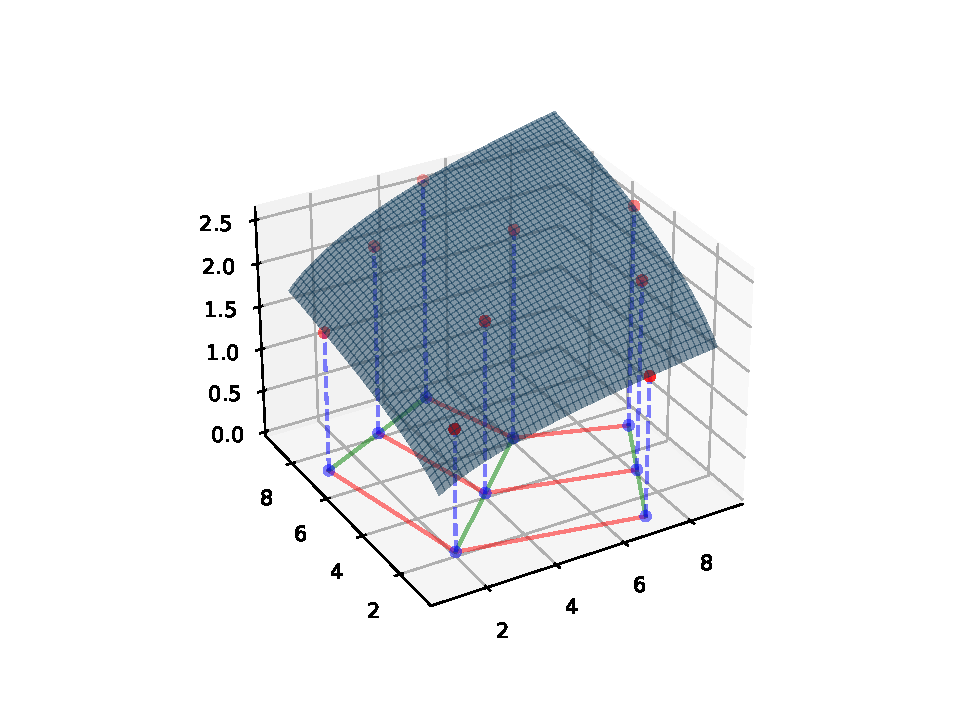
\includegraphics[width=0.7\linewidth]{files/WarpedInterpolation-408f6701cdebf478aa8559c8373a3025.pdf}
\caption{True function and curvilinear grid of points for which we know the value of the function.}
\label{fig:warped_interp}
\end{figure}

In Figure~\ref{fig:warped_interp}, we can see the true function in three-dimensional space, along with the points for which we actually know the value of the function. The underlying regular structure comes from the points' position in the matrix, the $(i,j)$ coordinates. If we join the points along every row and every column, we can see that the resulting grid is regular and piecewise affine (curvilinear).

In Figure~\ref{fig:homotopy} we see the values of the function at their index coordinate points in the matrix. We can see that there exists a mapping between the curvilinear grid and the index coordinates of the matrix.

\begin{figure}[!htbp]
\centering
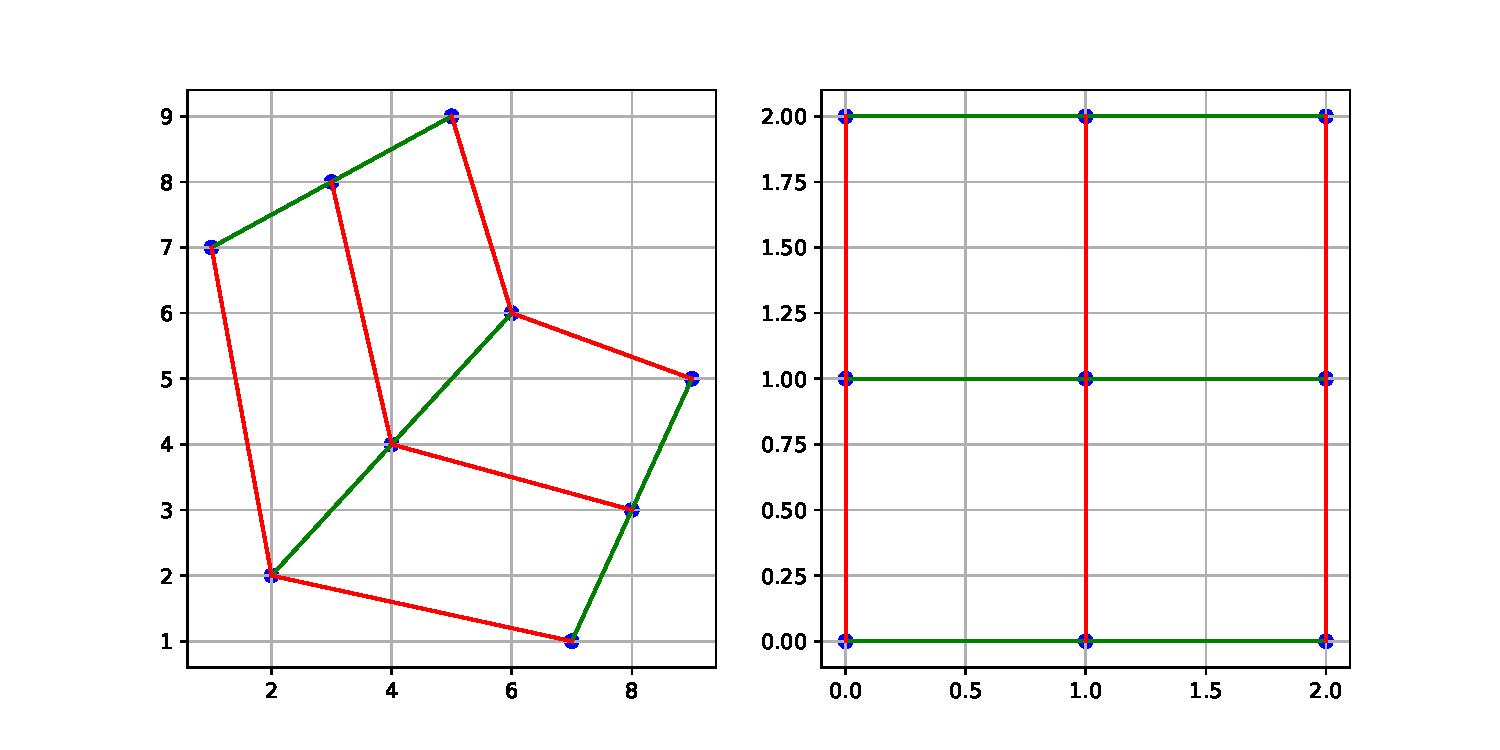
\includegraphics[width=0.7\linewidth]{files/Homotopy-d646f3c3fbd79fa1616ab23f185ea716.pdf}
\caption{Homotopy between the curvilinear grid and the index coordinates of the matrix.}
\label{fig:homotopy}
\end{figure}

The objective is to be able to interpolate the value of the function at any point off the grid, where presumably we are only interested in points internal to the curvilinear space and not outside the boundaries. For example, we can imagine that we want an approximation to the function at the point $(x,y) = (3, 5)$ pictured Figure~\ref{fig:mapping}. If we could find the corresponding point in the coordinate grid, interpolation would be straightforward. We can find where the $x$-coordinate of the point of interest intersects with the index-coordinates of the matrix. This is similar to assuming that we have 3 linear interpolators formed by connecting the points on the green lines in the x-direction, and for each interpolator we can approximate the corresponding y and z values using the grid data. Now, for each circle in Figure~\ref{fig:mapping}, we have a corresponding pair $(y,z)$, and we can interpolate in the y-direction to find the corresponding z-value for the point's y-coordinate\footnote{For more examples of the Warped Grid Interpolation method in action, see the github project\href{https://github.com/alanlujan91/multinterp/blob/main/notebooks/CurvilinearInterpolation.ipynb}{\texttt{alanlujan91/multinterp}}.}.

\begin{figure}[!htbp]
\centering
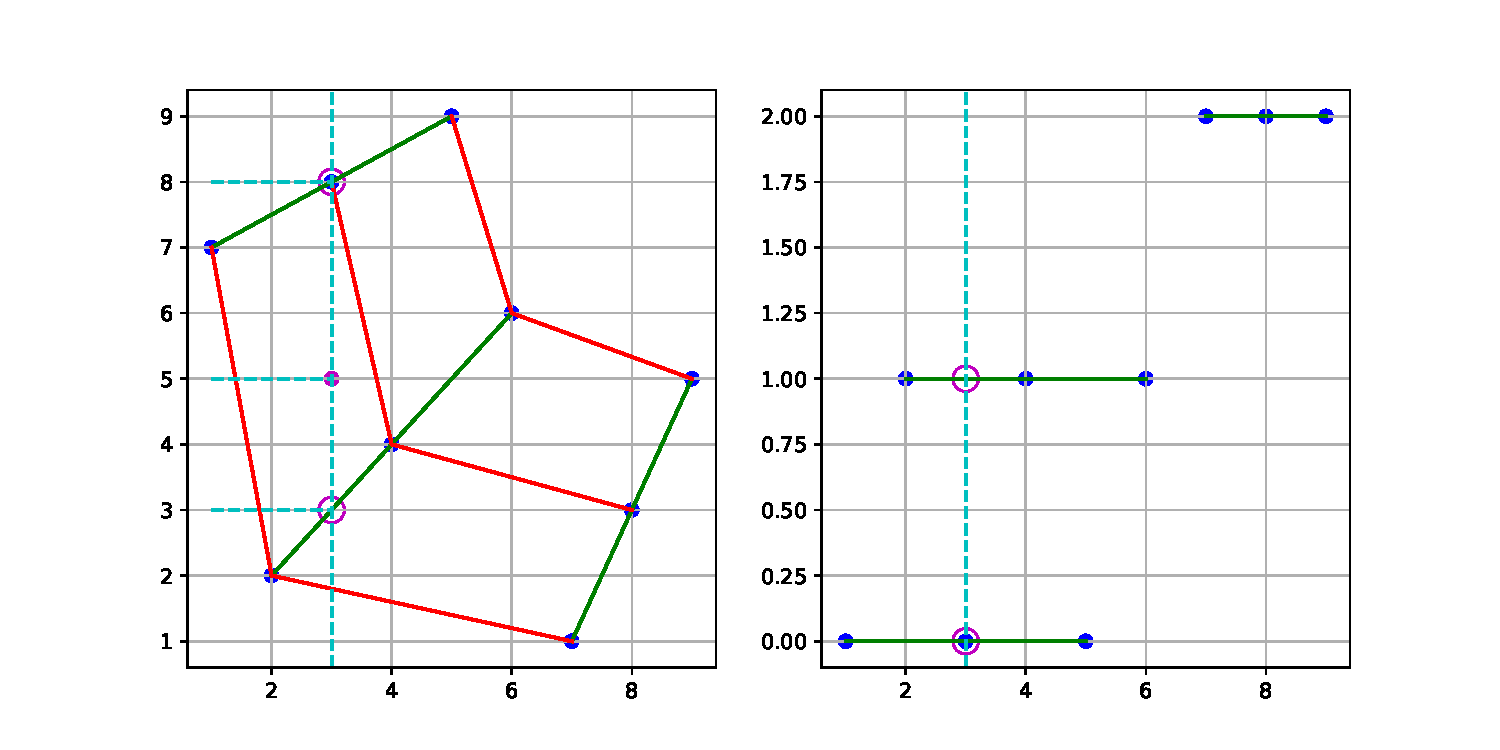
\includegraphics[width=0.7\linewidth]{files/Mapping-8901abed4cf13cf6f167297f87a8f27e.pdf}
\caption{The method consist of extending the loci of points in the $x$ dimension to find the corresponding crossing points in the $y$ dimension.}
\label{fig:mapping}
\end{figure}

\section{The EGM$^n$ in Higher Dimensions}\label{multdim}

The problem in Section~\ref{method} demonstrates the simplicity of solving problems sequentially. However, as constructed, the problem has only one state variable and one post-decision state variable per stage. Can EGM$^n$ be used to solve higher dimensional problems? In short, yes, but it requires additional thought on interpolation.

\subsection{A more complex problem}\label{A more complex problem}

For a demonstration, we now turn to the problem of a worker saving up for retirement. This worker must consume, save, and deposit resources into a tax-advantaged account that can not be liquidated until retirement. In the recursive problem, the worker begins a new period with a liquid account of market resources $\mRat_{t}$ and an illiquid account of retirement savings $\nRat_{t}$. The worker maximizes their utility by choosing consumption $\cRat_{t}$ and pension deposit $\dRat_{t}$. The pension deposit is set aside on a retirement account that is exposed to a risky return, while their post-consumption liquid assets accrue risk-free interest every period. The worker additionally receives an income that faces a permanent ($\PGro_{t+1}$) and a transitory ($\tShkEmp_{t+1}$) shock every period. At the age of 65, the worker is retired and their assets are liquidated, at which point the state reduces to one liquid account of market resources. The worker's recursive problem is:

\begin{equation}
\begin{split}
    \vFunc_{t}(\mRat_{t}, \nRat_{t}) & = \max_{\cRat_{t}, \dRat_{t}} \util(\cRat_{t}) + \DiscFac \Ex_{t} \left[ \PGro_{t+1}^{1-\CRRA} \vFunc_{t+1}(\mRat_{t+1}, \nRat_{t+1}) \right] \\
    & \text{s.t.} \quad \cRat_{t} \ge 0, \quad \dRat_{t} \ge 0 \\
    \aRat_{t} & = \mRat_{t} - \cRat_{t} - \dRat_{t} \\
    \bRat_{t} & = \nRat_{t} + \dRat_{t} + g(\dRat_{t}) \\
    \mRat_{t+1} & = \aRat_{t} \Rfree / \PGro_{t+1}  + \tShkEmp_{t+1} \\
    \nRat_{t+1} & = \bRat_{t} \Risky_{t+1} / / \PGro_{t+1}
  \end{split}
\end{equation}

where

\begin{equation}
\gFunc(\dRat) = \xFer \log(1+\dRat).
\end{equation}

This problem can subsequently be broken down into 3 stages: a pension deposit stage, a consumption stage, and an income shock stage.

\subsection{Breaking down the problem}\label{Breaking down the problem}

In the deposit stage, the worker begins with market resources and a retirement savings account. The worker must maximize their value of liquid wealth $\lRat_{t}$ and retirement balance $\bRat_{t}$ by choosing a pension deposit $\dRat_{t}$, which must be positive. The retirement balance $\bRat$ is the cash value of their retirement account plus their pension deposit and an additional amount $g(\dRat_{t})$ that provides an incentive to save for retirement. As we'll see, this additional term will allow us to use the Endogenous Grid Method to solve this subproblem.

\begin{equation}
\begin{split}
    \vFunc_{t}(\mRat_{t}, \nRat_{t}) & = \max_{\dRat_{t}} \vOpt_{t}(\lRat_{t}, \bRat_{t}) \\
    & \text{s.t.}  \quad \dRat_{t} \ge 0 \\
    \lRat_{t} & = \mRat_{t} - \dRat_{t} \\
    \bRat_{t} & = \nRat_{t} + \dRat_{t} + g(\dRat_{t})
  \end{split}
\end{equation}

After making their pension decision, the worker begins their consumption stage with liquid wealth $\lRat_{t}$ and retirement balance $\bRat_{t}$. From their liquid wealth, the worker must choose a level of consumption to maximize utility and continuation value $\wFunc_{t}$. After consumption, the worker is left with post-decision states that represent liquid assets $\aRat_{t}$ and retirement balance $\bRat_{t}$, which passes through this problem unaffected because it can't be liquidated until retirement.

\begin{equation}
\begin{split}
    \vOpt_{t}(\lRat_{t}, \bRat_{t}) & = \max_{\cRat_{t}} \util(\cRat_{t}) + \DiscFac \wFunc_{t}(\aRat_{t}, \bRat_{t})  \\
    & \text{s.t.} \quad \cRat_{t} \ge 0 \\
    \aRat_{t} & = \lRat_{t} - \cRat_{t}
  \end{split}
\end{equation}

Finally, the post-decision value function $\wFunc_{t}$ represents the value of both liquid and illiquid account balances before the realization of uncertainty regarding the risky return and income shocks. Since we are dealing with a normalized problem, this stage handles the normalization of state variables and value functions into the next period.

\begin{equation}
\begin{split}
    \wFunc_{t}(\aRat_{t}, \bRat_{t}) & = \Ex_{t} \left[ \PGro_{t+1}^{1-\CRRA} \vFunc_{t+1}(\mRat_{t+1}, \mRat_{t+1}) \right] \\
    & \text{s.t.} \quad \aRat_{t} \ge 0, \quad \bRat_{t} \ge 0 \\
    \mRat_{t+1} & = \aRat_{t} \Rfree / \PGro_{t+1}  + \tShkEmp_{t+1} \\
    \nRat_{t+1} & = \bRat_{t} \Risky_{t+1} /  \PGro_{t+1}
  \end{split}
\end{equation}

The advantage of conceptualizing this subproblem as a separate stage is that we can construct a function $\wFunc_{t}$ and use it in the prior optimization problems without having to worry about stochastic optimization and taking expectations repeatedly.

\subsection{The consumption-saving problem}\label{The consumption-saving problem}

As seen in the consumption stage above, the retirement balance $\bRat_{t}$ passes through the problem unaffected because it can't be liquidated until retirement. In this sense, it is already a post-decision state variable. To solve this problem, we can use a fixed grid of $\bRat_{t}$ and for each obtain endogenous consumption and ex-ante market resources using the simple Endogenous Grid Method for the consumption problem.

\subsection{The pension deposit problem}\label{The pension deposit problem}

In the deposit stage, both the state variables and post-decision variables are different since both are affected by the pension deposit decision.

First, we can rewrite the pension deposit problem more compactly:

\begin{equation}
\vFunc_{t}(\mRat_{t}, \nRat_{t}) = \max_{\dRat_{t}}
  \vOpt_{t}(\mRat_{t} - \dRat_{t}, \nRat_{t} + \dRat_{t} + \gFunc(\dRat_{t}))
\end{equation}

The first-order condition is

\begin{equation}
\vOpt_{t}^{\lRat}(\lRat_{t}, \bRat_{t})(-1) +
  \vOpt_{t}^{\bRat}(\lRat_{t}, \bRat_{t})(1+\gFunc'(\dRat_{t})) = 0.
\end{equation}

Rearranging this equation gives

\begin{equation}
\gFunc'(\dRat_{t}) = \frac{\vOpt_{t}^{\lRat}(\lRat_{t},
    \bRat_{t})}{\vOpt_{t}^{\bRat}(\lRat_{t}, \bRat_{t})} - 1
\end{equation}

where

\begin{equation}
\gFunc'(\dRat) =
  \frac{\xFer}{1+\dRat} \qquad \gFunc'^{-1}(y) = \xFer/y - 1
\end{equation}

Given that $\gFunc'(\dRat)$ exists and is invertible, we can find

\begin{equation}
\dEndFunc_{t}(\lRat_{t}, \bRat_{t}) = \gFunc'^{-1}\left(
  \frac{\vOpt_{t}^{\lRat}(\lRat_{t},
    \bRat_{t})}{\vOpt_{t}^{\bRat}(\lRat_{t},
    \bRat_{t})} - 1 \right)
\end{equation}

Using this, we can back out $\nRat_{t}$ as

\begin{equation}
\nEndFunc_{t}(\lRat_{t}, \bRat_{t}) = \bRat_{t} -
  \dEndFunc_{t}(\lRat_{t}, \bRat_{t}) - \gFunc(\dEndFunc_{t}(\lRat_{t},
    \bRat_{t}))
\end{equation}

and $\mRat_{t}$ as

\begin{equation}
\mEndFunc_{t}(\lRat_{t}, \bRat_{t}) = \lRat_{t} +
  \dEndFunc_{t}(\lRat_{t}, \bRat_{t})
\end{equation}

In sum, given an exogenous grid $(\lRat_{t}, \bRat_{t})$ we obtain the triple
$\left(\mEndFunc_{t}(\lRat_{t}, \bRat_{t}), \nEndFunc_{t}(\lRat_{t},
    \bRat_{t}), \dEndFunc_{t}(\lRat_{t}, \bRat_{t})\right)$, which
we can use to
create an interpolator for the decision rule $\dRat_{t}$.

To close the solution method, the envelope conditions are

\begin{equation}
\begin{split}
    \vFunc_{t}^{\mRat}(\mRat_{t}, \nRat_{t}) & =
    \vOpt_{t}^{\lRat}(\lRat_{t}, \bRat_{t}) \\
    \vFunc_{t}^{\nRat}(\mRat_{t}, \nRat_{t}) & =
    \vOpt_{t}^{\bRat}(\lRat_{t}, \bRat_{t})
  \end{split}
\end{equation}

\subsection{Unstructured Grid Interpolation}\label{Unstructured Grid Interpolation}

\begin{figure}[!htbp]
\centering
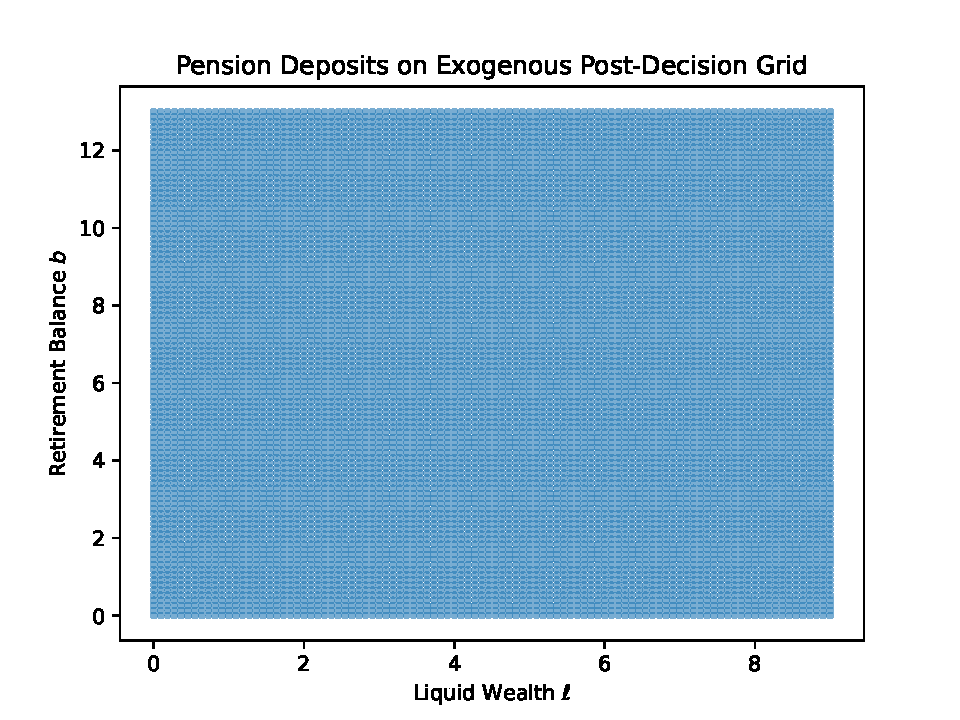
\includegraphics[width=0.7\linewidth]{files/ExogenousGrid-1327071c329af94ca01fc2e5abdd3eed.pdf}
\caption{A regular, rectilinear exogenous grid of pension balances after deposit $\bRat_{t}$ and liquid assets after consumption $\lRat_{t}$.}
\label{fig:exog}
\end{figure}

As in Section~\ref{method}, the resulting endogenous grid is not rectilinear, and in this more complex problem it is not even a regular grid. We can see in  Figure~\ref{fig:exog} that starting from a regular and rectilinear exogenous grid of liquid assets post-consumption $\lRat_{t}$ and pension balances post-deposit $\bRat_{t}$, we obtain Figure~\ref{fig:endog} which shows an irregular and unstructured endogenous grid of market resources $\mRat_{t}$ and pension balances pre-deposit $\nRat_{t}$.

\begin{figure}[!htbp]
\centering
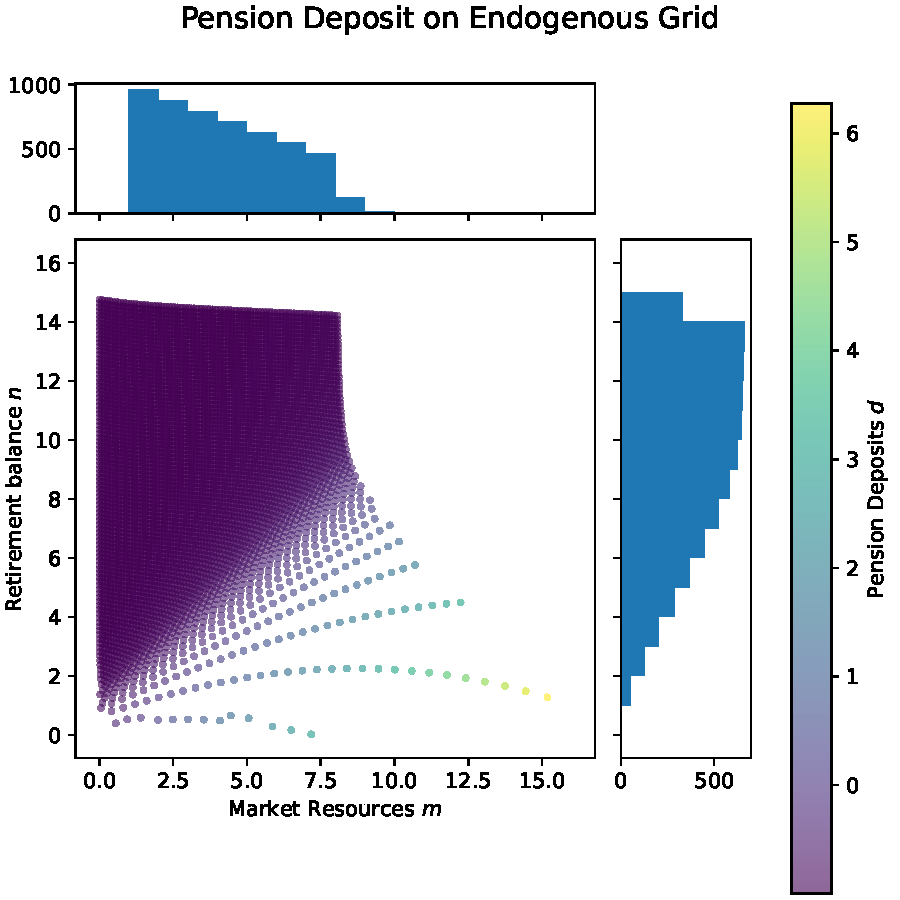
\includegraphics[width=0.7\linewidth]{files/EndogenousGrid-1ee13ab9f6b5410a9683ff5c35d8253e.pdf}
\caption{An irregular, unstructured endogenous grid of market resources $\mRat_{t}$ and pension balances before deposit $\nRat_{t}$.}
\label{fig:endog}
\end{figure}

To interpolate a function defined on an unstructured grid, we use Gaussian Process Regression as in \citet{Scheidegger2019}.

\section{Multivariate Interpolation on Unstructured Grids}\label{multinterp}

This section presents an alternative interpolation method for unstructured grids. I present a machine learning approach to interpolation on unstructured grids based on Gaussian Process Regression as presented in \citet{Scheidegger2019}.

\subsection{Unstructured Grids}\label{Unstructured Grids}

Unstructured interpolation arises in many dynamic programming applications when using the Endogenous Grid Method because the first-order conditions might be highly non-linear and non-monotonic, or because boundary constraints induce kinks in the policy and value functions. In these cases, the grid points generated by the EGM step are not evenly spaced, leading to the need for curvilinear interpolation. We saw in the previous subsection an approach to curvilinear interpolation based on \citet{White2015} that is incapable of interpolation on structured grids. A similar approach was presented in \citet{Ludwig2018} which used Delaunay interpolation. However, this approach is not well suited for our purposes because triangulation can be computationally intensive and slow, often offsetting the efficiency gains from the Endogenous Grid Method.

As an alternative to these methods, I introduce the use of Gaussian Process Regression (GPR) along with the Endogenous Grid Method. GPR is computationally efficient, and tools exist to easily parallelize and take advantage of hardware such as Graphics Processing Units (GPU)\footnote{\citet{Gardner2018}}.

% note: spell out GPU maybe or explain it in some way?

\subsection{Gaussian Process Regression}\label{Gaussian Process Regression}

A Gaussian Process is an infinite dimensional random process for which every subset of random variables is jointly Gaussian or has a multivariate normal distribution.

\begin{equation}
\begin{gathered}
    \mathbf{X} \sim \mathcal{N}(\mathbf{\mu}, \mathbf{\Sigma}) \quad \text{s.t.} \quad x_i \sim \mathcal{N}(\mu_i, \sigma_{ii}) \\
    \text{and} \quad  \sigma_{ij} = \Ex[(x_i - \mu_i)(x_j - \mu_j)] \quad \forall i,j \in \{1, \ldots, n\}.
  \end{gathered}
\end{equation}

where

\begin{equation}
\mathbf{X} = \begin{bmatrix}
    x_1    \\
    x_2    \\
    \vdots \\
    x_n
  \end{bmatrix}
  \quad
  \mathbf{\mu} = \begin{bmatrix}
    \mu_1  \\
    \mu_2  \\
    \vdots \\
    \mu_n
  \end{bmatrix}
  \quad
  \mathbf{\Sigma} = \begin{bmatrix}
    \sigma_{11} & \sigma_{12} & \cdots & \sigma_{1n} \\
    \sigma_{21} & \sigma_{22} & \cdots & \sigma_{2n} \\
    \vdots      & \vdots      & \ddots & \vdots      \\
    \sigma_{n1} & \sigma_{n2} & \cdots & \sigma_{nn}
  \end{bmatrix}.
\end{equation}

Being infinitely dimensional, a Gaussian Process can be used to represent a probability distribution over the space of functions in $n$ dimensions. Thus, a Gaussian Process Regression is used to find the best fit function to a set of data points.

\begin{equation}
\mathbb{P}(\mathbf{f} | \mathbf{X}) = \mathcal{N}(\mathbf{f} | \mathbf{m}, \mathbf{K})
\end{equation}

where $\mathbf{f}$ is the vector of function values at the points $\mathbf{X}$, $\mathbf{m}$ is the mean of the function, and $\mathbf{K}$ is a kernel function that describes the covariance between the function values at different points.

A standard kernel function is the squared exponential kernel, or the radial basis function kernel, which is defined as

\begin{equation}
k(\mathbf{x}_i, \mathbf{x}_j) = \sigma^2_f \exp\left(-\frac{1}{2l^2} (\mathbf{x}_i - \mathbf{x}_j)' (\mathbf{x}_i - \mathbf{x}_j)\right).
\end{equation}

Using GPR to interpolate a function $f$, we can both predict the value of the function at a point $\mathbf{x}_*$ and the uncertainty in the prediction, which provides useful information as to the accuracy of the approximation.

\subsection{An example of the GPR}\label{An example of the GPR}

In Figure~\ref{fig:true_function}, we see the function we are trying to approximate along with a sample of data points for which we know the value of the function. In practice, the value of the function is unknown and/or expensive to compute, so we must use a limited amount of data to approximate it.

\begin{figure}[!htbp]
\centering
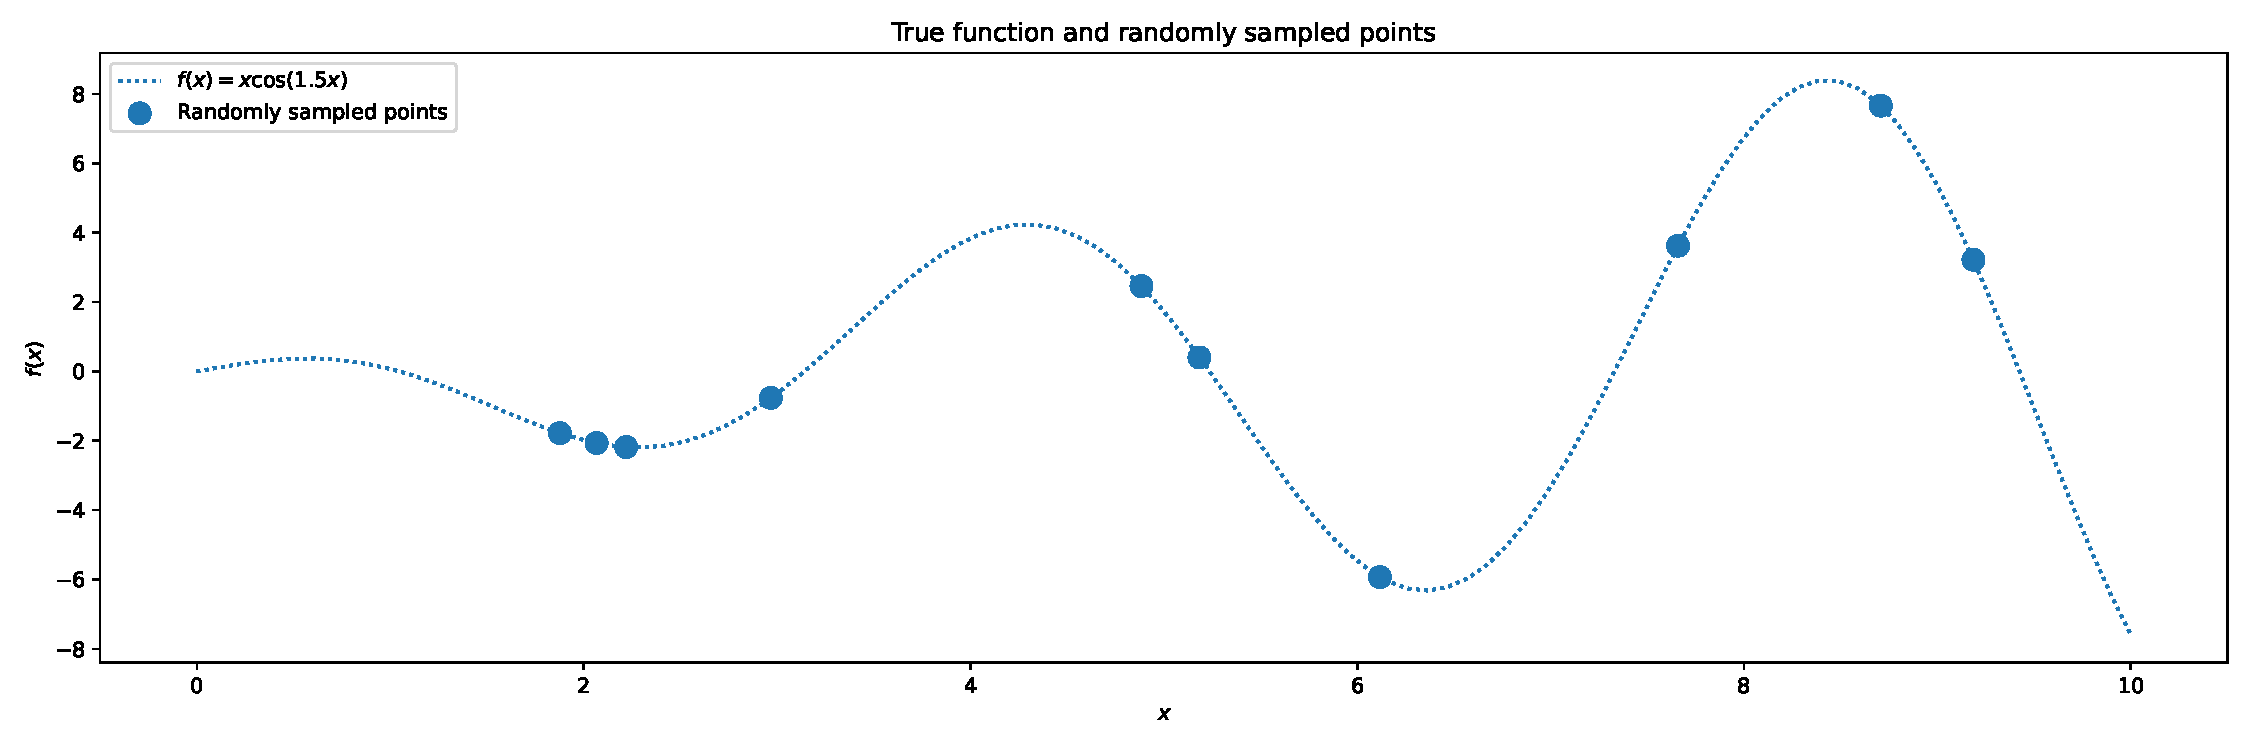
\includegraphics[width=0.7\linewidth]{files/true_function-35f17004b2f9b2f5acaedbaf5ee95879.pdf}
\caption{The true function that we are trying to approximate and a sample of data points.}
\label{fig:true_function}
\end{figure}

As we discussed, a Gaussian Process is an infinite dimensional random process which can be used to represent a probability of distributions over the space of functions. In Figure~\ref{fig:gpr_sample}, we see a random sample of functions from the GPR posterior, which is a Gaussian Process conditioned on fitting the data. From this small sample of functions, we can see that the GP generates functions that fit the data well, and the goal of GPR is to find the one function that best fits the data given some hyperparameters by minimizing the negative log-likelihood of the data.

\begin{figure}[!htbp]
\centering
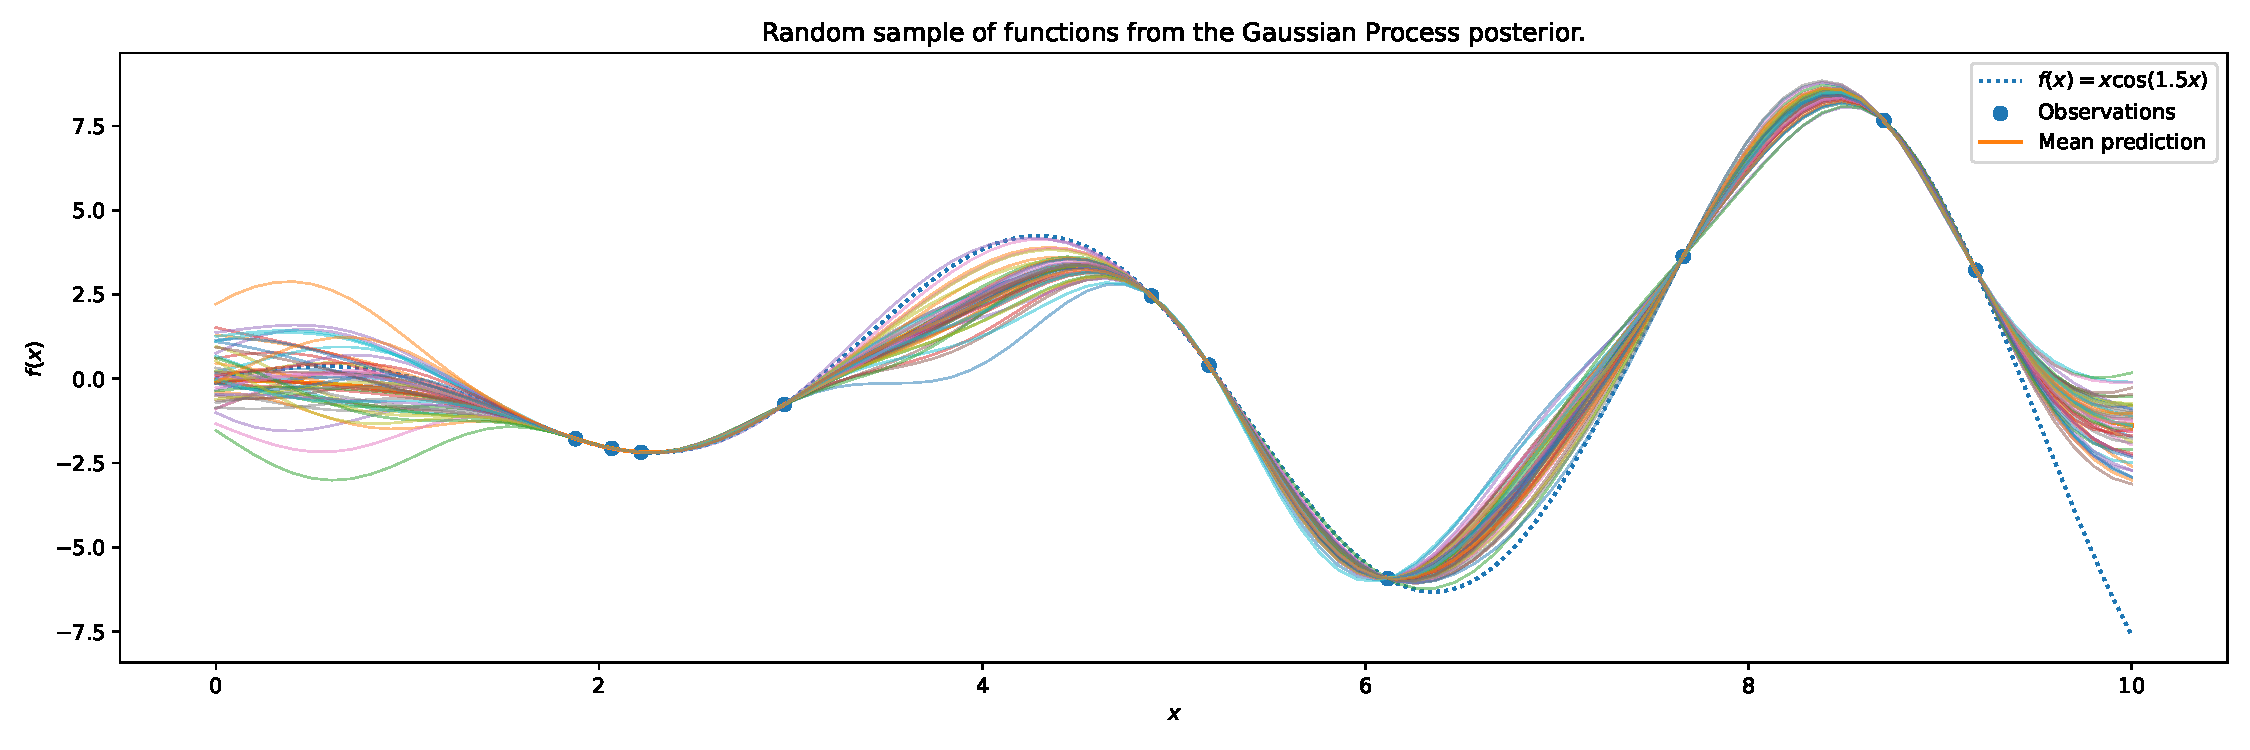
\includegraphics[width=0.7\linewidth]{files/gpr_sample-76cbb93ea31df5f08328cc0452b2f629.pdf}
\caption{A random sample of functions from the GPR posterior that fit the data. The goal of GPR is to find the function that best fits the data.}
\label{fig:gpr_sample}
\end{figure}

In Figure~\ref{fig:gpr}, we see the result of GPR with a particular parametrization\footnote{For details see notebook.} of the kernel function. The dotted line shows the true function, while the blue dots show the known data points. GPR provides the mean function which best fits the data, represented in the figure as an orange line. The shaded region represents a 95\% confidence interval, which is the uncertainty of the predicted function. Along with finding the best fit of the function, GPR provides the uncertainty of the prediction, which is useful information as to the accuracy of the approximation.

\begin{figure}[!htbp]
\centering
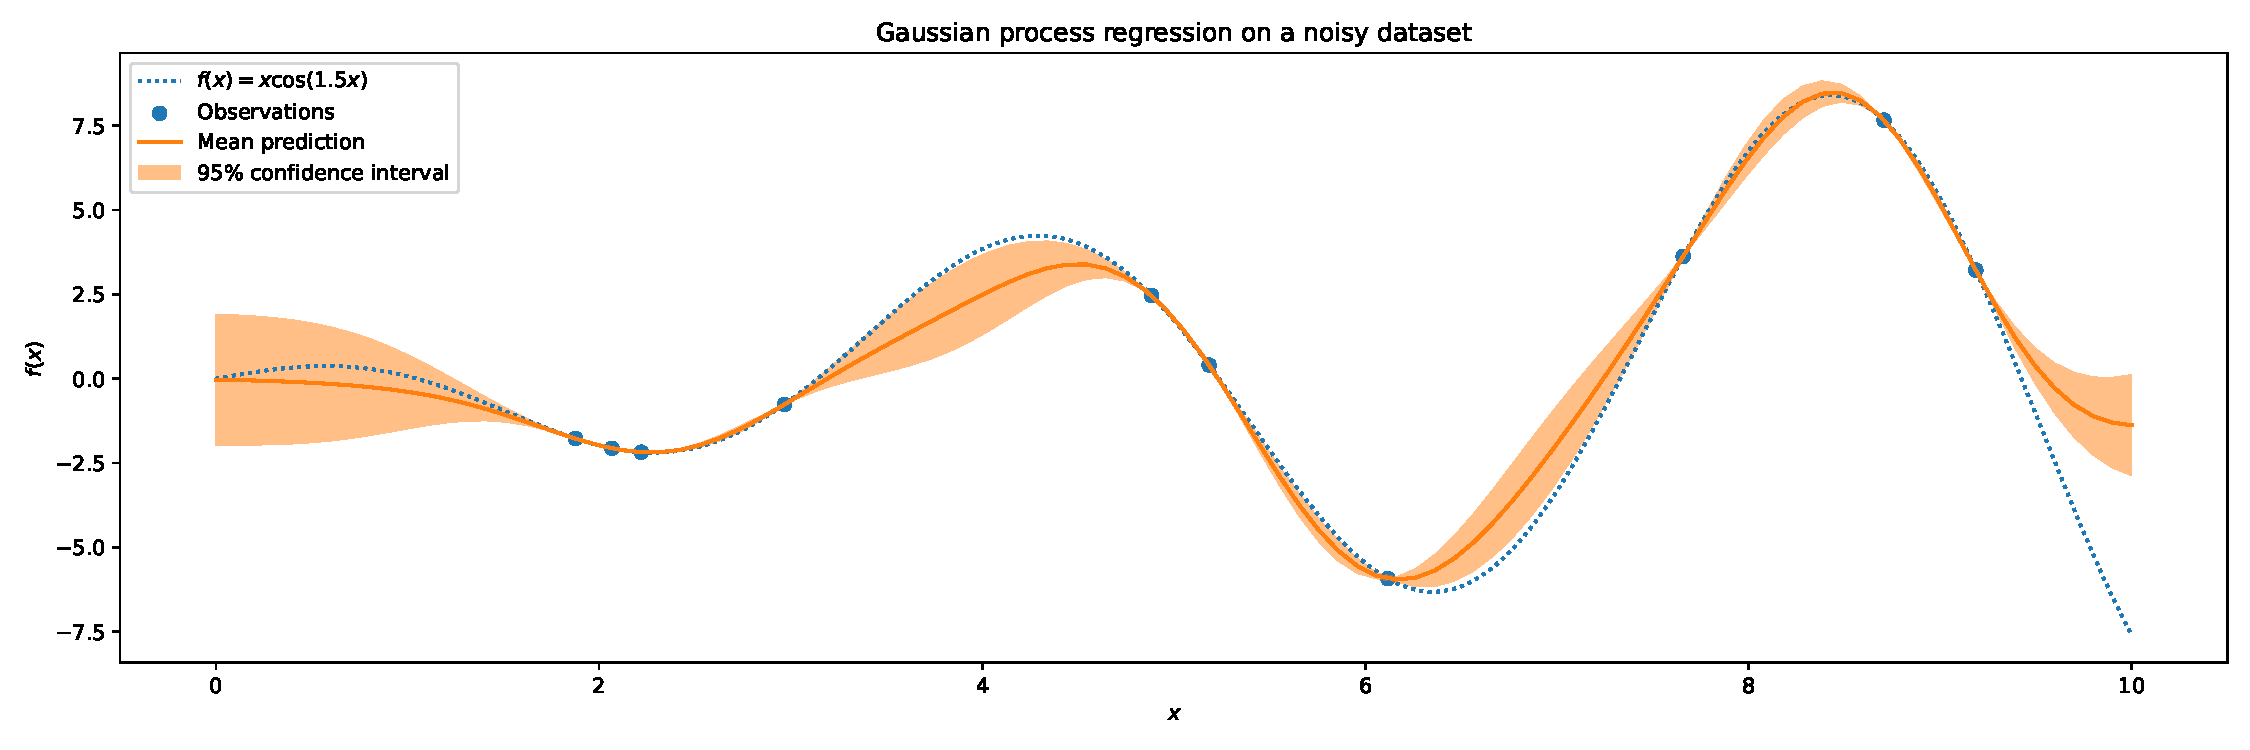
\includegraphics[width=0.7\linewidth]{files/gpr-2937ebcb72643a3aaed493f7141a76ce.pdf}
\caption{GPR finds the function that best fits the data given some hyperparameters. GPR then optimizes over the parameter space to find the function that minimizes the negative log-likelihood of the data.}
\label{fig:gpr}
\end{figure}

\section{Conditions for using the Sequential Endogenous Grid Method}\label{conditions}

\subsection{Splitting the problem into subproblems}\label{Splitting the problem into subproblems}

The first step in using the Sequential Endogenous Grid Method is to split the problem into subproblems. This process of splitting up the problem has to be strategic to not insert additional complexity into the original problem. If one is not careful when doing this, the subproblems can become more complex and intractable than the original problem.

% Comment: Need to decide if it is subproblem or subproblem # DONE

To split up the problem, we first count the number of control variables or decisions faced by the agent. Ideally, if the agent has $n$ control variables, then the problem should be split into $n$ subproblems, each handling a different control variable. For counting the number of control variables, it is important to not double count variables which are equivalent and have market clearing conditions. For example, the decision of how much to consume and how much to save may seem like two different choices, but because of the market clearing condition $\cRat + \aRat = \mRat$ they are resolved simultaneously and count as only one decision variable. Similarly, the
choice between labor and leisure are simultaneous and count as only one decision.

Having counted our control variables, we look for differentiable and invertible utility functions which are separable in the dynamic programming problem, such as in Section~\ref{method} of the paper, or differentiable and invertible functions in the transition, as in Section~\ref{multdim} of the paper.

% note: Capitalize Section for all instances # DONE

\subsubsection{Separable utility functions}\label{Separable utility functions}

In Section~\ref{method}, we have additively separable utility of consumption and leisure, which allows for each of these control variables to be handled by separate subproblems. So, it makes sense to split the utility between subproblems and attach one to the consumption subproblem and one to the leisure subproblem.

As mentioned in that section, however, there are only two separable utility functions in the problem which have been assigned to two subproblems already. This leaves one control variable without a separable utility function. In that case, there is not another Endogenous Grid Method step to exploit, and this subproblem has to be handled by standard convex optimization techniques such as maximization of the value function (VFI) or finding the root of the Euler equation (PFI).

% note: spell out small numbers except for when talking about a [Section %s](#multdim) etc

Now that we have split the problem into conceptual subproblems, it is important to sequence them in such a way that they don't become more complex than the original problem. The key here is to avoid adding unnecessary state variables. For example, in the consumption-leisure-portfolio problem, if we were to choose consumption first, we would have to track the wage rate into the following leisure subproblem. This would mean that our consumption problem would be two-dimensional as well as our labor decision problem. As presented, the choice of order in Section~\ref{method} ensures that the consumption problem is one-dimensional, as we can shed the information about the wage rate offer after the agent has made their labor-leisure decision. If we did this the other way, the problem would be more complex and require additional computational resources.

The consumption subproblem would be two-dimensional instead of one-dimensional, adding more complexity,

\begin{equation}
\begin{split}
        \vFunc(\bRat, \tShkEmp) & = \max_{\cRat} \uFunc(\cRat) + \vOpt(\bRat', \tShkEmp) \\
        & \text{s.t.}\\
        \bRat' & = \bRat - \cRat \ge - \tShkEmp
    \end{split}
\end{equation}

while the labor-leisure subproblem would have an additional constraint

\begin{equation}
\begin{split}
        \vOpt(\bRat', \tShkEmp) & = \max_{\leisure} \h(\leisure) + \vEnd(\aRat) \\
        & \text{s.t.} \\
        0 & \le \leisure \le 1 \\
        \aRat & = \bRat' + \tShkEmp(1 - \leisure) \ge 0.
    \end{split}
\end{equation}

Therefore, strategic ordering of subproblems can greatly simplify the solution process and reduce computational the burden.

\subsubsection{Differentiable and invertible transition}\label{Differentiable and invertible transition}

In Section~\ref{multdim}, we see that a problem with a differentiable and invertible transition can also be used to embed an additional Endogenous Grid Method step. Because the transition applies independently to a state variable that is not related to the other control variable, consumption, it can be handled separately from the consumption subproblem.

% note to check the tense of the entire text

In this particular problem, however, it turns out to make no difference how we order the two subproblems. This is because the control variables, consumption and pension deposit, each affect a separate resource account, namely market resources and pension balance. Because of this, the two subproblems are independent of each other and can be solved in any order.

A good rule of thumb is that when splitting up a problem into subproblems, we should try to reduce the information set that is passed onto the next subproblem. In Section~\ref{method}, choosing leisure-labor and realizing total market resources before consumption allows us to shed the wage rate offer state variable before the consumption problem, and we know that for the portfolio choice we only need to know liquid assets after expenditures (consumption). Thus, the order makes intuitive sense; agent first chooses leisure-labor, realizing total market resources, then chooses consumption and savings, and finally chooses their risky portfolio choice. In Section~\ref{multdim}, there are two expenditures that are independent of each other, consumption and deposit, and making one decision or the other first does not reduce the information set for the agent, thus the order of these subproblems does not matter.

\subsection{The Endogenous Grid Method for Subproblems}\label{The Endogenous Grid Method for Subproblems}

Once we have strategically split the problem into subproblems, we can use the Endogenous Grid Method in each applicable subproblem while iterating backwards from the terminal period. As we discussed in Sections Section~\ref{method} and Section~\ref{multdim}, the EGM step can be applied when there is a separable, differentiable and invertible utility function in the subproblem or when there is a differentiable and invertible transition in the subproblem. We will discuss each of these cases in turn.

\subsubsection{Utility function}\label{Utility function}

A generic subproblem with a differentiable and invertible utility function can be characterized as follows:

\begin{equation}
\begin{split}
        \VFunc(\xRat) &  = \max_{\yRat  \in \PGro(\xRat)} \UFunc(\xRat, \yRat) + \DiscFac \WFunc(\aRat) \\
        & \text{s.t.} \\
        \aRat & = \TFunc(\xRat,\yRat)
    \end{split}
\end{equation}

For an interior solution, the first-order condition is thus

\begin{equation}
\UFunc'_{\yRat}(\xRat, \yRat) + \DiscFac \WFunc'(\aRat)\TFunc'_{\yRat}(\xRat,\yRat) = 0
\end{equation}

If, as we assumed, the utility function is differentiable and invertible, then the Endogenous Grid Method consists of

\begin{equation}
\yRat = \left(\UFunc'_{\yRat}(\xRat, \yRat)\right)^{-1} \left[ -\DiscFac \WFunc'(\aRat)\TFunc'_{\yRat}(\xRat,\yRat)\right]
\end{equation}

By using an exogenous grid of the post-decision state $\aRat$, we can solve for the optimal decision rule $\yRat$ at each point on the grid. This is the Endogenous Grid Method step.

\subsubsection{Transition}\label{Transition}

If the generic subproblem has no utility, but instead has a differentiable and invertible transition, then the Endogenous Grid Method can still be used.

\begin{equation}
\begin{split}
        \VFunc(\xRat) &  = \max_{\yRat  \in \PGro(\xRat)}  \WFunc(\aRat) \\
        & \text{s.t.} \\
        \aRat & = \TFunc(\xRat,\yRat)
    \end{split}
\end{equation}

Here, the first-order condition is

\begin{equation}
\WFunc'(\aRat)\TFunc'_{\yRat}(\xRat,\yRat)  = 0
\end{equation}

and the Endogenous Grid Method step is

\begin{equation}
\yRat = \left(\TFunc'_{\yRat}(\xRat,\yRat)\right)^{-1} \left[ 1 / \WFunc'(\aRat)\right]
\end{equation}

\section{Conclusion}\label{conclusion}

% Summarize the method: Begin your conclusion by summarizing the new computational method you developed or proposed. Provide a brief overview of the key features of the method and how it differs from existing methods.

This paper introduces a novel method for solving dynamic stochastic optimization problems called the Sequential Endogenous Grid Method (EGM$^n$). Given a problem with multiple decisions (or control variables), the Sequential Endogenous Grid Method proposes separating the problem into a sequence of smaller subproblems that can be solved sequentially by using more than one EGM step. Then, depending on the resulting endogenous grid from each subproblem, this paper proposes different methods for interpolating functions on non-rectilinear grids, called the Warped Grid Interpolation (WGI) and the Gaussian Process Regression (GPR) method.

EGM$^n$ is similar to the Nested Endogenous Grid Method (NEGM)\footnote{\citet{Druedahl2021}.} and the Generalized Endogenous Grid Method (G2EGM)\footnote{\citet{Druedahl2017}.} in that it can solve problems with multiple decisions, but it differs from these methods in that by choosing the subproblems strategically, we can take advantage of multiple sequential EGM steps to solve complex multidimensional models in a fast and efficient manner. Additionally, the use of machine learning tools such as the GPR overcomes bottlenecks seen in unstructured interpolation using Delauany triangulation and other similar methods.

% Evaluate the method: Evaluate the strengths and limitations of the new computational method you developed or proposed. Discuss how the method compares to existing methods in terms of accuracy, efficiency, and ease of use.

% Demonstrate the method: If possible, provide an example of how the new computational method can be used to solve a problem or answer a research question. This will help the reader understand the practical implications of the method.

% Highlight potential applications: Discuss potential applications of the new computational method. This will help demonstrate the broader impact of the method beyond the specific problem or research question addressed in your paper.

% Discuss future directions: Provide suggestions for future research based on the new computational method you developed or proposed. This can include improvements to the method, potential extensions to other areas of research, or new applications of the method.

% Conclude with final thoughts: End your conclusion with some final thoughts that tie together the main points of your paper. This will help leave a lasting impression on the reader.

\section{Solving the illustrative G2EGM model with EGM$^n$}\label{appendix}

\subsection{The problem for a retired household}\label{The problem for a retired household}

I designate as $\wFunc_{t}(\mRat_{t})$ the problem of a retired household at time $t$ with total resources $\mRat$. The retired household solves a simple consumption-savings problem with no income uncertainty and a certain next period pension of $\underline{\tShkEmp}$.

\begin{equation}
\begin{split}
        \wFunc_{t}(\mRat_{t}) & = \max_{\cRat_{t}} \util(\cRat_{t}) +
        \DiscFac \wFunc_{t+1}(\mRat_{t}) \\
        & \text{s.t.} \\
        \aRat_{t} & = \mRat_{t} - \cRat_{t} \\
        \mRat_{t+1} & = \Rfree_{\aRat} \aRat_{t} +
        \underline{\tShkEmp}
    \end{split}
\end{equation}

Notice that there is no uncertainty and the household receives a retirement
income $\underline{\tShkEmp}$ every period until death.

\subsection{The problem for a worker household}\label{The problem for a worker household}

The value function of a worker household is

\begin{equation}
\VFunc_{t}(\mRat_{t}, \nRat_{t}) = \Ex_\error \max \left\{
    \vFunc_{t}(\mRat_{t}, \nRat_{t}, \Work) + \sigma_{\error}
    \error_{\Work} ,
    \vFunc_{t}(\mRat_{t}, \nRat_{t}, \Retire) + \sigma_{\error}
    \error_{\Retire} \right\}
\end{equation}

where the choice specific problem for a working household that decides to
continue working is

\begin{equation}
\begin{split}
        \vFunc_{t}(\mRat_{t}, \nRat_{t}, \Work) & = \max_{\cRat_{t},
            \dRat_{t}} \util(\cRat_{t}) - \kapShare + \DiscFac
        \Ex_{t} \left[
            \VFunc_{t+1}(\mRat_{t+1}, \nRat_{t+1})
            \right] \\
        & \text{s.t.} \\
        \aRat_{t} & = \mRat_{t} - \cRat_{t} - \dRat_{t} \\
        \bRat_{t} & = \nRat_{t} + \dRat_{t} + \gFunc(\dRat_{t}) \\
        \mRat_{t+1} & = \Rfree_{\aRat} \aRat_{t} + \tShkEmp_{t+1} \\
        \nRat_{t+1} & = \Rfree_{\bRat} \bRat_{t}
    \end{split}
\end{equation}

and the choice specific problem for a working household that decides to retire
is

\begin{equation}
\vFunc_{t}(\mRat_{t}, \nRat_{t}, \Retire) =
    \wFunc_{t}(\mRat_{t}+\nRat_{t})
\end{equation}

\subsection{Applying the Sequential EGM}\label{Applying the Sequential EGM}

The first step is to define a post-decision value function. Once the household
decides their level of consumption and pension deposits, they are left with
liquid assets they are saving for the future and illiquid assets in their
pension account which they can't access again until retirement. The
post-decision value function can be defined as

\begin{equation}
\begin{split}
        \vEnd_{t}(\aRat_{t}, \bRat_{t}) & =  \DiscFac
        \Ex_{t} \left[ \VFunc_{t+1}(\mRat_{t+1}, \nRat_{t+1}) \right] \\
        & \text{s.t.} \\
        \mRat_{t+1} & = \Rfree_{\aRat} \aRat_{t} + \tShkEmp_{t+1} \\
        \nRat_{t+1} & = \Rfree_{\bRat} \bRat_{t}
    \end{split}
\end{equation}

Then redefine the working agent's problem as

\begin{equation}
\begin{split}
        \vFunc_{t}(\mRat_{t}, \nRat_{t}, \Work) & = \max_{\cRat_{t},
            \dRat_{t}} \util(\cRat_{t})  - \kapShare + \vEnd_{t}(\aRat_{t},
        \bRat_{t}) \\
        \aRat_{t} & = \mRat_{t} - \cRat_{t} - \dRat_{t} \\
        \bRat_{t} & = \nRat_{t} + \dRat_{t} + \gFunc(\dRat_{t}) \\
    \end{split}
\end{equation}

Clearly, the structure of the problem remains the same, and this is the problem
that G2EGM solves. We've only moved some
of the stochastic mechanics out of the problem. Now, we can apply the
sequential EGM$^n$ method. Let the agent first decide $\dRat_{t}$, the deposit
amount into their retirement; we will call this the deposit problem, or outer loop. Thereafter, the
agent will have net liquid assets
of $\lRat_{t}$ and pension assets of $\bRat_{t}$.

\begin{equation}
\begin{split}
        \vFunc_{t}(\mRat_{t}, \nRat_{t}, \Work) & = \max_{\dRat_{t}}
        \vOpt_{t}(\lRat_{t}, \bRat_{t}) \\
        & \text{s.t.} \\
        \lRat_{t} & = \mRat_{t} - \dRat_{t} \\
        \bRat_{t} & = \nRat_{t} + \dRat_{t} + \gFunc(\dRat_{t})
    \end{split}
\end{equation}

Now, the agent can move on to picking their consumption and savings; we can call this
the pure consumption problem or inner loop.

\begin{equation}
\begin{split}
        \vOpt_{t}(\lRat_{t}, \bRat_{t}) & = \max_{\cRat_{t}}
        \util(\cRat_{t}) - \kapShare  + \vEnd_{t}(\aRat_{t}, \bRat_{t}) \\
        & \text{s.t.} \\
        \aRat_{t} & = \lRat_{t} - \cRat_{t} \\
    \end{split}
\end{equation}

Because we've already made the pension decision, the amount of pension assets
does not change in this loop and it just passes through to the post-decision
value function.

\subsection{Solving the problem}\label{Solving the problem}

\subsubsection{Solving the Inner Consumption Saving Problem}\label{Solving the Inner Consumption Saving Problem}

Let's start with the pure consumption-saving problem, which we can summarize by
substitution as

\begin{equation}
\vOpt_{t}(\lRat_{t}, \bRat_{t}) = \max_{\cRat_{t}} \util(\cRat_{t}) - \kapShare +
    \vEnd_{t}(\lRat_{t} - \cRat_{t}, \bRat_{t})
\end{equation}

The first-order condition is

\begin{equation}
\util'(\cRat_{t}) = \vEnd_{t}^{\aRat}(\lRat_{t}-\cRat_{t}, \bRat_{t}) =
    \vEnd_{t}^{\aRat}(\aRat_{t}, \bRat_{t})
\end{equation}

We can invert this Euler equation as in standard EGM to obtain the consumption
function.

\begin{equation}
\cEndFunc_{t}(\aRat_{t}, \bRat_{t}) =
    \util'^{-1}\left(\vEnd_{t}^{\aRat}(\aRat_{t}, \bRat_{t})\right)
\end{equation}

Again as before, $\lEndFunc_{t}(\aRat_{t}, \bRat_{t}) =
    \cEndFunc_{t}(\aRat_{t}, \bRat_{t}) + \aRat_{t}$. To sum up, using an
exogenous
grid of $(\aRat_{t}, \bRat_{t})$ we obtain the trio $(\cEndFunc_{t}(\aRat_{t},
    \bRat_{t}), \lEndFunc_{t}(\aRat_{t},
    \bRat_{t}), \bRat_{t})$ which
provides an
interpolating function for our optimal consumption decision rule over the
$(\lRat, \bRat)$ grid. Without loss of generality, assume $\lEndFunc_{t} =
    \lEndFunc_{t}(\aRat_{t}, \bRat_{t})$ and define the interpolating
function as

\begin{equation}
\cTarg_{t}(\lEndFunc_{t}, \bRat_{t}) \equiv \cEndFunc_{t}(\aRat_{t},
    \bRat_{t})
\end{equation}

For completeness, we derive the envelope conditions as well, and as we will
see, these will be useful when solving the next section.

\begin{equation}
\begin{split}
        \vOpt_{t}^{\lRat}(\lRat_{t}, \bRat_{t}) & =
        \vEnd_{t}^{\aRat}(\aRat_{t}, \bRat_{t}) = \util'(\cRat_{t}) \\
        \vOpt_{t}^{\bRat}(\lRat_{t}, \bRat_{t}) & =
        \vEnd_{t}^{\bRat}(\aRat_{t}, \bRat_{t})
    \end{split}
\end{equation}

\subsubsection{Solving the Outer Pension Deposit Problem}\label{Solving the Outer Pension Deposit Problem}

Now, we can move on to solving the deposit problem, which we can also summarize
as

\begin{equation}
\vFunc_{t}(\mRat_{t}, \nRat_{t}, \Work) = \max_{\dRat_{t}}
    \vOpt_{t}(\mRat_{t}
    - \dRat_{t}, \nRat_{t} + \dRat_{t} + \gFunc(\dRat_{t}))
\end{equation}

The first-order condition is

\begin{equation}
\vOpt_{t}^{\lRat}(\lRat_{t}, \bRat_{t})(-1) +
    \vOpt_{t}^{\bRat}(\lRat_{t}, \bRat_{t})(1+\gFunc'(\dRat_{t})) = 0
\end{equation}

Rearranging this equation gives

\begin{equation}
\gFunc'(\dRat_{t}) = \frac{\vOpt_{t}^{\lRat}(\lRat_{t},
        \bRat_{t})}{\vOpt_{t}^{\bRat}(\lRat_{t}, \bRat_{t})} - 1
\end{equation}

Assuming that $\gFunc'(\dRat)$ exists and is invertible, we can find

\begin{equation}
\dEndFunc_{t}(\lRat_{t}, \bRat_{t}) = \gFunc'^{-1}\left(
    \frac{\vOpt_{t}^{\lRat}(\lRat_{t},
        \bRat_{t})}{\vOpt_{t}^{\bRat}(\lRat_{t},
        \bRat_{t})} - 1 \right)
\end{equation}

Using this, we can back out $\nRat_{t}$ as

\begin{equation}
\nEndFunc_{t}(\lRat_{t}, \bRat_{t}) = \bRat_{t} -
    \dEndFunc_{t}(\lRat_{t}, \bRat_{t}) - \gFunc(\dEndFunc_{t}(\lRat_{t},
        \bRat_{t}))
\end{equation}

and $\mRat_{t}$ as

\begin{equation}
\mEndFunc_{t}(\lRat_{t}, \bRat_{t}) = \lRat_{t} +
    \dEndFunc_{t}(\lRat_{t}, \bRat_{t})
\end{equation}

In sum, given an exogenous grid $(\lRat_{t}, \bRat_{t})$ we obtain the triple
$\left(\mEndFunc_{t}(\lRat_{t}, \bRat_{t}), \nEndFunc_{t}(\lRat_{t},
        \bRat_{t}), \dEndFunc_{t}(\lRat_{t}, \bRat_{t})\right)$, which
we can use to
create an interpolator for the decision rule $\dRat_{t}$.

To close the solution method, the envelope conditions are

\begin{equation}
\begin{split}
        \vFunc_{t}^{\mRat}(\mRat_{t}, \nRat_{t}, \Work) & =
        \vOpt_{t}^{\lRat}(\lRat_{t}, \bRat_{t}) \\
        \vFunc_{t}^{\nRat}(\mRat_{t}, \nRat_{t}, \Work) & =
        \vOpt_{t}^{\bRat}(\lRat_{t}, \bRat_{t})
    \end{split}
\end{equation}

\subsection{Is g invertible?}\label{Is g invertible?}

We've already seen that $\util'(\cdot)$ is invertible, but is $\gFunc$?

\begin{equation}
\gFunc(\dRat) = \xFer \log(1+\dRat) \qquad \gFunc'(\dRat) =
    \frac{\xFer}{1+\dRat} \qquad \gFunc'^{-1}(y) = \xFer/y - 1
\end{equation}

\subsection{The Post-Decision Value and Marginal Value Functions}\label{The Post-Decision Value and Marginal Value Functions}

\begin{equation}
\begin{split}
        \vEnd_{t}(\aRat, \bRat) & =  \DiscFac \Ex_{t} \left[
            \VFunc(\mRat_{t+1}, \nRat_{t+1}) \right] \\
        & \text{s.t.} \\
        \mRat_{t+1} & = \Rfree_{\aRat} \aRat_{t} + \tShkEmp_{t+1} \\
        \nRat_{t+1} & = \Rfree_{\bRat} \bRat_{t}
    \end{split}
\end{equation}

and

\begin{equation}
\begin{split}
        \vEnd_{t}^{\aRat}(\aRat_{t}, \bRat_{t}) & =  \DiscFac
        \Rfree_{\aRat} \Ex_{t} \left[ \VFunc^{\mRat}_{t+1}(\mRat_{t+1},
            \nRat_{t+1})
            \right] \\
        & \text{s.t.} \\
        \mRat_{t+1} & = \Rfree_{\aRat} \aRat_{t} + \tShkEmp_{t+1} \\
        \nRat_{t+1} & = \Rfree_{\bRat} \bRat_{t}
    \end{split}
\end{equation}

and

\begin{equation}
\begin{split}
        \vEnd_{t}^{\bRat}(\aRat_{t}, \bRat_{t}) & =  \DiscFac
        \Rfree_{\bRat} \Ex_{t} \left[ \VFunc^{\nRat}_{t+1}(\mRat_{t+1},
            \nRat_{t+1})
            \right] \\
        & \text{s.t.} \\
        \mRat_{t+1} & = \Rfree_{\aRat} \aRat_{t} + \tShkEmp_{t+1} \\
        \nRat_{t+1} & = \Rfree_{\bRat} \bRat_{t}
    \end{split}
\end{equation}

\subsection{Taste Shocks}\label{Taste Shocks}

From discrete choice theory and from DCEGM paper, we know that

\begin{equation}
\Ex_{t} \left[
        \VFunc_{t+1}(\mRat_{t+1}, \nRat_{t+1}, \error_{t+1}) \right] =
    \sigma \log \left[ \sum_{\Decision \in \{\Work, \Retire\}} \exp \left(
        \frac{\vFunc_{t+1}(\mRat_{t+1}, \nRat_{t+1},
            \Decision)}{\sigma_\error} \right)  \right]
\end{equation}

and

\begin{equation}
\Prob_{t}(\Decision ~ \lvert ~ \mRat_{t+1}, \nRat_{t+1}) = \frac{\exp
        \left(
        \vFunc_{t + 1}(\mRat_{t+1}, \nRat_{t+1}, \Decision) /
        \sigma_\error
        \right)
    }{  \sum\limits_{\Decision \in \{\Work, \Retire\}} \exp \left(
        \frac{\vFunc_{t+1}(\mRat_{t+1}, \nRat_{t+1},
            \Decision)}{\sigma_\error} \right)}
\end{equation}

the first-order conditions are therefore

\begin{equation}
\vOptAlt_{t}^{\mRat}(\mRat_{t+1}, \nRat_{t+1}) = \sum_{\Decision \in
        \{\Work, \Retire\}} \Prob_{t}(\Decision ~
    \lvert ~
    \mRat_{t+1}, \nRat_{t+1}) \vFunc_{t+1}^{\mRat}(\mRat_{t+1},
    \nRat_{t+1},
    \Decision)
\end{equation}



        \bibliographystyle{unsrtnat}
    \bibliography{main.bib}

\end{document}
